\documentclass{sig-alternate}
\usepackage[ruled,vlined,linesnumbered]{algorithm2e}
\usepackage{algpseudocode}
\usepackage{amsmath}
\usepackage{amssymb}
\usepackage{bm}
\usepackage{bbding}
\usepackage{caption}
\usepackage{color}
\usepackage{enumitem}
\usepackage{epsfig}
\usepackage{ifpdf}
\usepackage[Large]{subfigure}
\usepackage{tikz}
\usepackage{verbatim}
\usepackage{pgfplots}
\usepackage{float}
\usepackage{soul}
\usepackage{makecell}
\usepackage{pgfplotstable}
\usepackage{booktabs}
\usepackage{colortbl}
\usepackage{longtable}
%\usepackage[dvipsnames]{xcolor}
%\usepackage{authblk}


\usetikzlibrary{arrows,calc,shapes,snakes,automata,backgrounds,fit,petri,patterns}

\ifpdf
  \DeclareGraphicsRule{*}{mps}{*}{}
\fi

%\allowdisplaybreaks
%
%\setlength{\oddsidemargin}{4mm}
%\setlength{\evensidemargin}{\oddsidemargin}
%\setlength{\textwidth}{160mm}
%\setlength{\topmargin}{-5.4mm}
%\setlength{\headheight}{5mm}
%\setlength{\headsep}{5mm}
%\setlength{\footskip}{10mm}
%\setlength{\textheight}{230mm}
%
%\def\figures{0}

\newcommand{\norm}[1]{\ensuremath{\left\| #1 \right\|}}
\newcommand{\dataset}{\mathcal{D}}

% A pointer for comments
\def\pointer{\HandRight $\phantom{0}$}

% Math operators
\def\argmax{\operatornamewithlimits{arg\,max}}
\def\argmin{\operatornamewithlimits{arg\,min}}
\def\const{\mathop{\rm const}}
\def\cov{\mathop{\rm cov}}
\def\tr{\mathop{\sf tr}}
\def\trace{\mathop{\sf trace}}
\def\var{\mathop{\sf var}}

% Users and items. I think "item" is already a keyword.
\def\usr{\mathop{\rm user}}
\def\itm{\mathop{\rm item}}

% Double bold
\def\Ebb{\mathbb{E}}
\def\Ibb{\mathbb{I}}
\def\Rbb{\mathbb{R}}
\def\Xbb{\mathbb{X}}

% Bold Greek
\def\balpha{\bm{\alpha}}
\def\bbeta{\bm{\beta}}
\def\bmeta{\bm{\eta}}
\def\bgamma{\bm{\gamma}}
\def\bGamma{\mathbf{\Gamma}}
\def\blambda{\bm{\lambda}}
\def\bLambda{\mathbf{\Lambda}}
\def\bmu{\bm{\mu}}
\def\bnu{\bm{\nu}}
\def\bOmega{\mathbf{\Omega}}
\def\bpi{\bm{\pi}}
\def\bPi{\mathbf{\Pi}}
\def\bSigma{\mathbf{\Sigma}}
\def\btau{\bm{\tau}}
\def\btheta{\bm{\theta}}
\def\bTheta{\mathbf{\Theta}}
\def\bxi{\bm{\xi}}
\def\bzeta{\bm{\zeta}}

% Normal bold
\def\0{\mathbf{0}}
\def\a{\mathbf{a}}
\def\b{\mathbf{b}}
\def\c{\mathbf{c}}
\def\d{\mathbf{d}}
\def\e{\mathbf{e}}
\def\f{\mathbf{f}}
\def\k{\mathbf{k}}
\def\m{\mathbf{m}}
\def\r{\mathbf{r}}
\def\s{\mathbf{s}}
\def\u{\mathbf{u}}
\def\v{\mathbf{v}}
\def\w{\mathbf{w}}
\def\x{\mathbf{x}}
\def\y{\mathbf{y}}
\def\z{\mathbf{z}}
\def\A{\mathbf{A}}
\def\B{\mathbf{B}}
\def\C{\mathbf{C}}
\def\D{\mathbf{D}}
\def\E{\mathbf{E}}
\def\F{\mathbf{F}}
\def\G{\mathbf{G}}
\def\H{\mathbf{H}}
\def\I{\mathbf{I}}
\def\J{\mathbf{J}}
\def\K{\mathbf{K}}
\def\L{\mathbf{L}}
\def\P{\mathbf{P}}
\def\R{\mathbf{R}}
\def\S{\mathbf{S}}
\def\U{\mathbf{U}}
\def\V{\mathbf{V}}
\def\W{\mathbf{W}}
\def\X{\mathbf{X}}
\def\Y{\mathbf{Y}}
\def\Z{\mathbf{Z}}

\def\parent{\texttt{par}}
\def\children{\texttt{child}}


% Brackets
\def\<{ \left\langle }
\def\>{ \right\rangle }

% Caligraphic
\def\Bcal{\mathcal{B}}
\def\Dcal{\mathcal{D}}
\def\Ecal{\mathcal{E}}
\def\Fcal{\mathcal{F}}
\def\Gcal{\mathcal{G}}
\def\Hcal{\mathcal{H}}
\def\Ical{\mathcal{I}}
\def\Lcal{\mathcal{L}}
\def\Mcal{\mathcal{M}}
\def\Ncal{\mathcal{N}}
\def\Ocal{\mathcal{O}}
\def\Rcal{\mathcal{R}}
\def\Scal{\mathcal{S}}
\def\Tcal{\mathcal{T}}
\def\Zcal{\mathcal{Z}}

% General
\def\erm{\mathrm{e}}
\def\wo{\backslash}
\def\defined{\stackrel{\text{\tiny def}}{=}}
\newcommand{\bigE}[1]{{ \big\langle {#1} \big\rangle }}
\newcommand{\BigE}[1]{{ \Big\langle {#1} \Big\rangle }}
\newcommand{\BiggE}[1]{{ \Bigg\langle {#1} \Bigg\rangle }}

\definecolor{Blue}{rgb}{0.0,0.0,1.0}
\newcommand{\bluetext}[1]{{\color{Blue}{#1}}}

\definecolor{White}{rgb}{1.0,1.0,1.0}
\newcommand{\whitetext}[1]{{\color{White}{#1}}}

\def\checkmark{\tikz\fill[scale=0.4](0,.35) -- (.25,0) -- (1,.7) -- (.25,.15) -- cycle;} 

\pgfplotsset{compat=1.11,
    /pgfplots/ybar legend/.style={
    /pgfplots/legend image code/.code={%
       \draw[##1,/tikz/.cd,yshift=-0.25em,]
        (0cm,0cm) rectangle (10pt,1.8em);},
   },
}

\setlength{\textfloatsep}{5pt plus 1.0pt minus 2.0pt}

\makeatletter
\renewcommand{\paragraph}{\@startsection{paragraph}{4}{\z@}%
  {-2.25ex\@plus -1ex \@minus -.2ex}%
  {0.5ex \@plus .2ex}%
  {\normalfont\normalsize\bfseries}}

\makeatother


\newcommand{\todo}[1]{\ifnum\comments>0{\color{Blue}{[UP: #1]}}\fi} 
\newcommand{\SBE}[1]{\ifnum\comments>0{\sethlcolor{green}{\hl{[SBE: #1]}}}\fi} 
\newcommand{\GL}[1]{\ifnum\comments>0\hl{[GL: #1]}\fi }
\newcommand{\noam}[1]{\ifnum\comments>0{\color{purple}{[NK: #1]}}\fi} 



\def\comments{0}
\def\fsize{9}


\title{Groove Radio: A Bayesian Hierarchical Model for Personalized Playlist Generation}

\begin{document}

%\newcounter{exercisecounter}
%\noindent \Large \textsf{Radio Paper Outline}
%\normalsize
%\hfill\textsf{Shay, Hilik, Noam, Oren, Tal and Gal}
%\hfill\textsf{\today}
%\noindent\rule{\textwidth}{2pt}
%\vspace{4pt}
%\noindent using the bootcamp \LaTeX  template

%\numberofauthors{6}
%\author{
%	\alignauthor
%	Author 1\\
%	\affaddr{Affiliation}
%	\alignauthor
%	Author 2\\
%	\affaddr{Affiliation}
%	\alignauthor
%	Author 3\\
%	\affaddr{Affiliation}
%	\and
%	\alignauthor
%	Author 4\\
%	\affaddr{Affiliation}
%	\alignauthor
%	Author 5\\
%	\affaddr{Affiliation}
%	\alignauthor
%	\and
%	Author 6\\
%	\affaddr{Affiliation}
%	\alignauthor
%	Author 7\\
%	\affaddr{Affiliation}
%}

\numberofauthors{1}
\author{
	\alignauthor
	Anonymous Authors\\
	\affaddr{Affiliation}
	\alignauthor
}



\maketitle

%\vspace{-2mm}
\begin{abstract}
	This paper describes an algorithm designed for Microsoft's Groove music service, which serves millions of users world wide.  We consider the problem of automatically generating personalized music playlists based on queries containing a ``seed'' artist and the listener's user ID. 
Playlist generation may be informed by a number of data sources including: listening patterns, genre taxonomy, acoustic features, and popularity. The importance assigned to each of these information sources may vary depending on the specific combination of user and ``seed" artist.

The paper presents a method based on a variational Bayes solution for learning the parameters of a model containing a four-level hierarchy of global preferences, genres, sub-genres and artists. The proposed model further incorporates a personalization component for user-specific preferences.
Empirical evaluations on both private and public datasets demonstrate the effectiveness of the algorithm and showcase the contribution of each of its components.\GL{Moved to intro: An online A/B experiment, comparing this algorithm to Groove's previous playlist algorithm, shows an increase in user listening time as well as a reduction in the number of skipped tracks.}

%The problem of automatic playlist generation is at the core of the intersection between recommender systems and the music domain. 
%Microsoft's Groove music service offers automatic playlists based on a ``seed'' artist and listener history, serving millions of users world-wide. 
\SBE{I want to propose a more engaging first paragraph: The problem of automatic playlist generation is at the core of the intersection between recommender systems and the music domain. Microsoft's Groove music service offers automatic playlists based on a ``seed'' artist and listener history, serving millions of users world-wide. etc.}\GL{Looks good to me, lets integrate it and start converging on a final version} \noam{please no. I really liked the old version. what can be more engaging than a description of a real world system? Besides, the MIR community is small and sometimes looked down upon by outsiders due their high acceptance rate policy.}

\end{abstract}
%\vspace{-2mm}     
\section{Introduction}
\label{sec:Introduction}
   %!TEX root = RadioPaper_Main.tex
Online music services such as Spotify, Pandora, Google Play Music and Microsoft's Groove serve as a major growth engine for today's music industry. A key experience is the ability to stream automatically generated playlists based on some criteria chosen by the listener.
%Scenarios such as genre, artist and track-based radio are tasked with creating audio playlists which suit user tastes and can be several hours long, based on limited explicit input from the user. 
This paper considers the problem of automatically generating personalized music playlists based on queries containing a ``seed'' artist and the listener's user ID \SBE{I feel that this is too repetitive across the paper.}\GL{IMO this is preferable to having the reader be lost looking for definitions in the intro while reading the model}. We describe a solution designed for Microsoft's Groove internet radio \SBE{removed quotation marks from radio to be consistent with title} service, which serves playlists to millions of users world wide. 
%This model was implemented and compared to Groove's previous playlist solution using an online experiment showing an increase in users' listening time and a reduction in the number of skipped tracks.

In recommender systems research, collaborative filtering approaches such as matrix factorization are often used to learn relations between users and items \cite{KorenBV09}. 
The playlist generation task is essentially different as it requires learning a coherent sequence to allow smooth track transitions.
Central to the approach taken in this research is the idea of estimating the relatedness of a ``candidate'' track to the previously selected tracks already in the playlist.
%A Naive approach might select one particular type of similarity (e.g. tracks from the same genre or tracks from the same era) and return all appropriate tracks according to this measure.  
%Moreover, matrix factorization approaches are based on learning latent features using on one type of information source typically explicit ratings or implicit usage patterns. 
Such relatedness can depend on multiple information sources, such as meta-data and domain semantics, the acoustic audio signal,  and popularity patterns, as well as information extracted using collaborative filtering techniques.  
%Meta-data similarity is defined by the semantics of two tracks. %(e.g. both tracks are recorded by the same artist). 
%Usage similarity is defined by the consumption patterns of two tracks (e.g. users who listened to one also listened to the other) and can be learned using collaborative filtering methods such as matrix factorization. Acoustic similarity is extracted by digital signal processing on the audio signal.% of two tracks (e.g. they both contain drums and piano). 
%Beyond similarity, consumption patterns of commercial music are also inherently trendy. That is, popular tracks may be a welcome addition to a playlist regardless of their similarity to other tracks in the list. 

The multiplicity of useful signals has motivated recent works  \cite{personalized_playlist_schedl,McFee_multi_similarities} to combine several information sources in order to model playlists. % and provide a more robust estimate of relatedness.  
While it is known that all these factors play a role in the construction of a quality playlist, a key distinction of Groove's model is the idea that the importance of each of these information sources varies depending on the specific seed artist. For example, when composing a playlist for a Jazz artist such as John Coltrane, the importance of acoustic similarity features may be high. In contrast, in the case of a contemporary pop artist, such as Lady Gaga, features based on collaborative filtering may be more important. In Section~\ref{sec:experiments}, evaluations are provided in support of this assumption.
 
Another key element of the model in this paper is personalization based on the listener. For example, a particular user may prefer strictly popular tracks, while another prefers more esoteric content. %Yet another user may prefer music from a particular genre or artist. 
Our method provides for modeling user specific preferences via personalization components.


%This taxonomy allows to capture variance in the importance of features at different levels of the hierarchy. For example, the variance between subgenres in the ``World Music'' genre could possibly be much greater than other genres such as Rock music, due to the eclectic nature of the former. Thus, our model would learn the necessary  sub-genre or even artist level distinction between the factors that should be applied to construct the playlist.

The model in this paper is designed to support any artist in Groove's catalog, far beyond the small number of artists that dominate the lion's share of user listening patterns. The distribution of artists in the catalog contains a long tail of less popular artists for which insufficient information exists to learn artist specific parameters. Therefore, the Groove model also leverages the hierarchical taxonomy of genres, sub-genres and artists, native to the music domain. %I omitted album and tracks since these are not parts of the hierarchy in our model. Feel free to revert. 
When particular artists or possibly even sub-genres are underrepresented in the data, the Groove model can still allow prediction by ``borrowing'' information from sibling nodes sharing the same parent in the taxonomy. %Similarly, our model also affords  ``cold users" the benefit of the learned domain taxonomy parameters, allowing construction of a quality playlist upon their very first launch of the service. 

%This  paper proposes a novel machine learning approach encapsulating the above attributes. 
The Groove model casts playlist construction as a classification problem: predicting the next track given the seed artist, the user ID, and previously played tracks. 
As such, a hierarchical Bayesian model is suggested to perform playlist prediction using logistic regression. 
%This approach is essentially different from most collaborative filtering algorithms in which there is no 
%Specifically, the four-level hierarchy of global preferences, genres, sub-genres, and artists. 
Parameter learning follows the variational Bayes approach of approximating the posterior distribution using a probability distribution which factorizes over the parameters. 
%We evaluate our approach on two datasets, each representing a slightly different type of signal. The Groove music dataset, represents explicit skip data. That is, negative examples in this dataset are explicitly provided by users.
%\todo{We should be careful of the ``dataset shift'' issue, where explicitly provided negative data are a function of our
%current model. For the sake of the reviewers, we should have an answer about the feedback loop and biases, as the negatives are not i.i.d.\ldots}\GL{ I tried to adress this in the practical considerations section, do you think more is needed on this point?}
%The 30Music dataset \cite{DBLP:conf/recsys/TurrinQCPC15}, is a dataset of user compiled playlists. In this dataset, the negatives are implied. They are sampled from those tracks that do not appear \GL{not sure what 'together' means here} on a user defined playlist. 
%In this type of signal, the semantic hierarchy is able to perform nearly as well as the personalization.
The evaluation of this model demonstrates the contribution of the hierarchical domain taxonomy and the personalization components to the prediction task at hand. 
%We are able to achieve AUC of 0.9 and 0.86 for the two datasets, respectively. We also provide an analysis of the benefit afforded by considering different sets (and combinations of) similarity feature types, as well as an analysis of the robustness of our approach to user and item ``coldness" \SBE{need to be consistent in placing this term in quotation marks} \GL{we need to make sure to synchronize this passage in case any changes are made to the experiments section}. 
Beyond this evaluation, the performance of a production variant of approach described in this paper was validated in an online A/B experiment. The experiment shows an increase in user listening time and a reduction in the number of skipped tracks relative to the experiment baseline.


%Our paper is organized as follows: Section \ref{sec:Related} discusses relevant related work. Section \ref{sec:OurModel} motivates our approach, discusses the specification of our model and explains the  algorithm we apply to learn the parameters from data. Section \ref{sec:Features} describes the features we use to encode  playlist context. Section \ref{sec:experiments} gives the details of our experimental evaluation. Section \ref{sec:PracticalConsiderations} describes additional modifications that allow the proposed approach to work in large-scale scenarios. Finally, section \ref{sec:conclusion} summarizes our results.



%\vspace{-2mm}
\section{Related Work}
\label{sec:Related}
    %!TEX root = RadioPaper_Main.tex
Automatic playlist generation is an active research field. The formulation of the playlist generation problem varies across literature and, consequently, various types of methods and evaluations are proposed \cite{playlist_survey}.	This problem is mainly researched in the domains of Recommender Systems research and Music Information Retrieval (MIR). 

  	
Recommender systems excel at learning relations between users and items (personalization).
Specifically, predicting music ratings in the presence of a genre taxonomy was the focus of the 2011 KDD-Cup competition \cite{KDD_Cup11}. In \cite{Dror2011}, a matrix factorization model was presented in which the domain taxonomy was utilized in order to propagate information between parameters with shared ancestors in the taxonomy (e.g. tracks belonging to the same artist etc). As explained earlier, this paper addresses a very different problem: finding the next track to be added to a playlist in the context of an artist seed, the user ID and previously played tracks. Unlike matrix factorization methods, it is not based on learning latent features. Instead, it builds upon multiple explicit information sources that include collaborative filtering along with meta-data, acoustic signals and popularity patterns. In essence, it is a hybrid approach \cite{Hybrid_recsys} that builds upon similarities derived from various sources. It can also be viewed as a two-layered cascade in which different algorithms are utilized in the first layer to produce various types of similaritiy that serve as features to a second layer that produces the playlist. As such it bears resemblance to a recent paper on optimizing click-through rate in recommender systems \cite{www2016}.  

% and in learning item similarities at the level of tracks, artists and albums. %and are designed to produce recommendations according to a specific user taste. 
In the music domain, similarities are typically derived from: 
usage \cite{item2vec,Mcfee_learningsimilarity_CF}, meta-data \cite{Bogdanov_content,  McfeeEtAl_2009_HeteEmbeForSubj, Pauws:ISMIR02,SlaneyEtAl_2008_LearAMetrFor} or both \cite{a2mf}.  Yet, producing good similarities between tracks is not always sufficient for generating high quality playlists \cite{playlist_survey}.
Section~\ref{sec:Features} provides an overview of the features used in this paper. 
However, the focus of this work is on the underlying algorithm for generating the playlists given these similarities.
	
		
In MIR research, different approaches for playlist generation have been proposed. Typically, tracks are ranked based on audio features, meta-data and specific user queries \cite{DoplerEtAl_2008_AcceMusiCollVia, Lee2011}. %The method proposed in this work both has a model of state and utilizes multiple sources of information and thus can be  considered a combination of recommendation system and MIR approaches.	
Learning from multiple types of similarity was investigated in \cite{McFee_multi_similarities}, where the authors propose a method for integrating heterogeneous data into a single similarity space. Our method differs from \cite{McFee_multi_similarities} in several aspects: First, it is able to utilize the hierarchical semantic structure that exists in the taxonomy of the music domain. Second, it is formalized as a binary classification problem, whereas the method in \cite{McFee_multi_similarities} produces embedding in a latent space. Third, it contains a personalization component and generates playlists according to a specific combination of artist and user. Additionally, it provides a measure of confidence in the predictions inherent to Bayesian modeling.
	
Hierarchical classification models are well studied in the literature \cite{Cai2004,NIPS2012_4609, Zhou2011}. Hierarchical MIR models are proposed in \cite{DecoroEtAl_2007_BayeAggrForHier, Dror2011,Pampalk2005} for the applications of genre classification,  music recommendations, and artist organization, respectively. To the best of our knowledge, this paper is the first to introduce a Bayesian hierarchical model that utilizes both multiple sources and the domain taxonomy at various resolutions (genre, sub-genre and artist) for the application of automatic personalized playlist generation. 

% NK - the below section does not strengthen the paper since I beleive it makes our eveluation section pale with respect to some of these approaches	
%Several different types of playlist evaluations exist: Human evaluation \cite{Barrington2009, Pauws:ISMIR02} measures the user feedback to a played playlist. Semantic cohesion \cite{Logan2002, Logan2004} uses tags and metadata in order to measure the coherence between the played tracks and hence the cohesion of the playlist as a whole. Sequence prediction \cite{ MailletEtAl_2009_SteePlayGeneBy,Mcfee2011} aims at predicting the next song that is most suitable to be played in a specific context. This type of evaluation requires positively and negatively labeled examples, that can be established using either ``plays" and ``skips" \cite{EliasPampalkTimTimPohle2005} or `plays' and uniform sampling. In this work, we apply sequence prediction evaluation according to a specific state that depends on a combination of multiple user related and artist related features. \GL{ I'm not sure about this passage, is classification accuracy really the same as sequence prediction? If so we need to update the experiment section to say as much}
	

%\vspace{-2mm}    
\section{Modeling Contextual\\ Playlists}
\label{sec:ourapproach}
    %!TEX root = RadioPaper_Main.tex
\label{sec:OurModel}
As was previously stated, the algorithm in this paper is designed to generate personalized playlists in the context of a seed artist and a specific user. In Groove music, a playlist request named ``radio'' can be called by each subscriber using any artist in the catalog as a seed. An artist seed is a common scenario in many alternative online music services, but the algorithm in this paper can be extended to support also track seeds, genre seeds, seeds based on labels as well as various combinations of the above, called ``multi-seeds". In this paper we limit the discussion to the case of a single artist seed.

As explained earlier, constructing a playlist depends on multiple similarities used in estimating the relatedness of a new candidate track to the playlist. These similarities are based on meta-data, usage, acoustic features, and popularity patterns. 
%Another important feature group contains features based on the popularity of a candidate track. \GL{The above sentences closely resemble the intro} 
However, the importance of each feature may be different for each seed. To account for difference in the importance of features for different seed artists, we propose a model which incorporates per-artist parameters that capture this variance. In the presence of a user with historical listening data, the quality of the playlist may be further improved with personalization. Hence, the proposed model includes additional parameters that enable encoding per-user preferences. 

A design goal of the proposed model is to support new or unknown users and/or seed artists which are new or ``cold" (i.e. sparsely represented in the training data). If there is insufficient information on the user, the proposed model performs a graceful fall-back, relying only on parameters related to the seed artist. In the case of an unknown or ``cold" artist, the proposed model relies on the hierarchical domain taxonomy to allow a graceful fall-back using the parameters at the sub-genre level. This property applies also to underrepresented sub-genres and even genres, afforded by relying on correspondingly higher levels in the domain taxonomy. 


The algorithm constructs a playlist by iteratively picking the next track to be added to the playlist. 
At each stage, the algorithm considers candidate tracks to be added to the playlist and predicts their relatedness to the seed, previously selected tracks and the user. 
Previously selected tracks, together with seed artist and user information, constitute the ``context'' from which the model is trained to predict the next track to play. This context is encoded as a feature vector, as described in Section~\ref{sec:Features}.  

%The information that relates the candidate track to seed, the existing tracks and the user is encoded as a feature vector called 

%To facilitate learning transitions in the playlist, the choice of the next track to be played is made using knowledge of the tracks that were previously selected. 

\subsection{Playlists as a Classification Problem}
\label{sec:playlist_is_classification}
We denote by $\x_i \in \mathbb{R}^d$ the context feature vector representing the proposition of suggesting a particular track $i$ at a particular ``context'' of previous playlist tracks, a seed artist and the user.\GLw{Added following ulrich's commnet..} Note that the features encoded in $\x_i$  will vary between different candidate tracks even if they belong to the same artist or genre.  These context feature vectors are mapped to a binary label $r_i \in \{0,1\}$,where $r_i=1$ indicates a positive outcome for the proposition and $r_i=0$ indicates a negative outcome. Thus, we have reduced our problem of playlist selection to a classification problem.

The dataset is denoted by $\mathcal{D}$ and consists of context vectors paired with labeled outcomes, denoted by the tuples $\left(\x_i,r_i\right) \in \mathcal{D}$.
The binary labels may encode different real-world outcomes  given the context. 
For example, in a dataset collected from playlist data logs, a track  played to its conclusion may be considered a positive outcome ($r_i=1$), whereas a track  skipped  mid-play may be considered a negative outcome ($r_i=0$). Alternatively, consider a dataset of user-compiled collections. Tracks appearing in a collection may be considered positive outcomes, while some sample of catalog tracks not appearing in the collection are considered negative outcomes.  In Section~\ref{sec:experiments} we provide an evaluation using both of these approaches. 


\subsection{The Model}
In what follows, we describe a  hierarchical Bayesian classification model enriched with additional personalization parameters. We also provide a learning algorithm that generalizes the dataset $\mathcal{D}$ and enables generation of new playlists.

\subsubsection{Notation}
We discern vectors and matrices from scalars by denoting the former in {\bf bold} letters. We further discern the vectors from the matrices by using lowercase letters for the vectors and capital letters for matrices. For example, $x$ is a scalar, $\x$ is a vector and $\X$ is a matrix. We denote by $\I$ the identity matrix and $\0$ represents a vector of zeros. 


The  domain taxonomy is represented as a tree-structured graphical model. Each artist in the catalog corresponds to a leaf-node in the tree, with a single parent node corresponding to the artist's sub-genre. Similarly, each node corresponding to a sub-genre has a single parent node representing the appropriate genre. All nodes corresponding to genres  have a single parent, the root node of the tree. We denote by $\parent(n)$ and $\children(n)$ the mappings from a node indexed by $n$ to its parent and to the set of its children, respectively. We denote by $G$, $S$, $A$ and $U$ the total number of genres, sub-genres, artists and users, respectively. 

We denote by $N$ the size of $\mathcal{D}$, our dataset.
For the $i$'th tuple in $\mathcal{D}$, we denote by $g_i$, $s_i$, $a_i$ and $u_i$ the specific genre, sub-genre, artist and user corresponding to this datum, respectively.
Finally, $\w^{(g)}_{g_i}$, $\w^{(s)}_{s_i}$, $\w^{(a)}_{a_i}$, $\w^{(u)}_{u_i}$,
$\w \in\mathbb{R}^d$ denote the parameters for genre $g_i$, sub-genre $s_i$, artist $a_i$, user $u_i$, and the root, respectively.

\subsubsection{Likelihood}
We model the probability of a single example $(\x_i, r_i) \in \mathcal{D}$ given the context vector $\x_i$,
the artist parameters $\w^{(a)}_{a_i}$ and the user parameters $\w^{(u)}_{u_i}$  as:
%%
%% \GL{Not sure equations being so tiny saves so much space, see comparison below, ive added a parameter \\fsize at the top of the doc and set it to 9(instead of 7), the equations look slightly more readable to me}
% \begin{equation}
% \begingroup\makeatletter\def\f@size{\fsize}
% \begin{aligned}
% p\left( r_i \mid \x_i , \w^{(a)}_{a_i}, \w^{(u)}_{u_i} \right) & = \left[ \sigma \left( \x_i^\top \left( \w^{(a)}_{a_i} + \w^{(u)}_{u_i} \right) \right) \right]^{r_i} \\ 
% &  \hspace{0mm} \cdot \left[ 1- \sigma \left( \x_i^\top \left( \w^{(a)}_{a_i} + \w^{(u)}_{u_i} \right) \right) \right]^{(1-r_i)},
% \label{eq:likelihood}
% \end{aligned}\endgroup
% \end{equation}
\begin{align}
 p( r_i | \x_i , \w^{(a)}_{a_i}, \w^{(u)}_{u_i} )
& =  \big[ \sigma \big( \x_i^\top ( \w^{(a)}_{a_i} + \w^{(u)}_{u_i} ) \big) \big]^{r_i} \nonumber \\ 
& \ \:  \cdot \big[ 1 - \sigma \big( \x_i^\top ( \w^{(a)}_{a_i} + \w^{(u)}_{u_i} ) \big) \big]^{(1-r_i)} ,
\label{eq:likelihood}
\end{align}
%%
where  $\sigma(x) \defined (1 + \mathrm{e}^{-x})^{-1}$ denotes the logistic function.
The likelihood of the dataset $\mathcal{D}$ is simply the product of these probabilities i.e., $\prod_i p( r_i | \x_i , \w^{(a)}_{a_i}, \w^{(u)}_{u_i})$.

%, under the assumptions that the labels $r_i$ are i.i.d.
% [NK]  - The i.i.d assumption is obvious. No need to explicitly mention it. A reviewer might question it which may actually be a problem in our case. Better not mention it...

%\todo{One question that people might ask is why the model is additive, e.g.~why the $w$-vectors are added. We could say something like, if we concatenated our features $[\x_i, \x_i]$ and weights $[\w^{(a)}_{a_i}, \w^{(u)}_{u_i}]$, so that the interaction are modelled separately between users and features, and another context and features, then this linear model is exactly what we have above, etc.}
%\SBE{Another insight to Ulrich's comment that we can say is related to the way we train th model, we alternate between parameters, starting from the hierarchy, thereby learning users as a vector difference from artists, this way artists are sort of a prior when there is no information on users. WDYT?} \GL{I'm not sure  this is the right place to discuss these matters, this being the section were we state the model plainly. Perhaps a small passage at the top of section 3}

\subsubsection{Hierarchical Prior}
The prior distribution over the user parameters is a multivariate Gaussian:
$p(\w^{(u)}_{u_i} | \tau_u) = \mathcal{N}(\w^{(u)}_{u_i} ; \0, \tau_u^{-1}\I )$, where $\tau_u$ is a precision parameter.
The prior distribution over the global, genre, sub-genre, and artist parameters applies the domain taxonomy to define a hierarchy of priors as follows:
%\begin{equation}
%\begingroup\makeatletter\def\f@size{\fsize}
%\begin{aligned}
%&p\left(\w^{(a)}_{a_i} \mid \w^{(s)}_{s_i}, \tau_a\right) = \mathcal{N}\left(\w^{(a)}_{a_i}; \w^{(s)}_{s_i}, \tau_a^{-1}\I \right), \\
%&p\left(\w^{(s)}_{s_i} \mid \w^{(g)}_{g_i}, \tau_s\right) = \mathcal{N}\left(\w^{(s)}_{s_i}; \w^{(g)}_{g_i}, \tau_s^{-1}\I \right), \\
%&p\left(\w^{(g)}_{g_i} \mid \w, \tau_g\right) = \mathcal{N}\left(\w^{(g)}_{g_i}; \w, \tau_g^{-1}\I \right), \\
%&p\left(\w \mid \tau_w \right) = \mathcal{N}\left(\w; \0, \tau_w^{-1}\I \right),
%\label{eq:priors}
%\end{aligned}\endgroup
%\end{equation}
\begin{align}
&p(\w^{(a)}_{a_i} | \w^{(s)}_{s_i}, \tau_a )  = \mathcal{N} (\w^{(a)}_{a_i}; \w^{(s)}_{s_i}, \tau_a^{-1}\I ) \ , \nonumber \\
&p(\w^{(s)}_{s_i} | \w^{(g)}_{g_i}, \tau_s)   = \mathcal{N} (\w^{(s)}_{s_i}; \w^{(g)}_{g_i}, \tau_s^{-1}\I ) \ , \nonumber \\
&p(\w^{(g)}_{g_i} | \w, \tau_g )              = \mathcal{N} (\w^{(g)}_{g_i}; \w, \tau_g^{-1}\I )             \ , \nonumber \\
&p(\w | \tau_w)                               = \mathcal{N} (\w; \0, \tau_w^{-1}\I ) \ ,
\end{align}
%%
where $\tau_a, \tau_s, \tau_g$, $\tau_w$ are scalar precision parameters.
This prior structure allows sibling artists (belonging to the same sub-genre) to propagate information through the common sub-genre parameters. 
In case of a ``cold'' artist, it allows borrowing information from siblings by initializing the artist parameters according to the sub-genre parameters (i.e. ``warm'' initialization). As more information on the artist is observed, its parameters can gradually shift away from the prior position to a more accurate representation based on the observed data.
%to be encoded in relation to their sub-genres, and the sub-genres parameters to be encoded in relation to genres.
%As an energy function (log joint density), a smaller penalty is paid by encoding two similar artists \emph{once} in their sub-genre;
These arguments follow along the hierarchical structure and apply to the sub-genre and genre parameters as well.
% [NK] - We do not have latent representaitons here. This is not matrix factorizaton. All we got is priors on weight paramters that can borrow information from sibling nodes. Also, it is not true that the aritst is only an "extension" of the prior. The entire vector is encoded.
%\todo{We should tie this to different choices of hierarchy, in the experimental results.}
%\todo{Can we add an ``embedding visualisation'', a bit like in Noam and my Xbox Movies paper? It helps to bring the point home!}\GL{its not clear what we would see in such a visualization, perhaps clustering of sub-genres around their genre? im not too sure what to expect across genres, as we dont have a classification problem here that incentivizes clear separation of the classes}

We define a set of hyper-priors over the precision parameters given by:
%\begin{equation}
%\begingroup\makeatletter\def\f@size{\fsize}\check@mathfonts
%\def\maketag@@@#1{\hbox{\m@th\large\normalfont#1}}%
%\begin{aligned}
%&p\left( \tau_u \mid \alpha, \beta \right) = \mathcal{G}\left(\tau_u ; \alpha, \beta \right), 
%\qquad p\left( \tau_a \mid \alpha, \beta \right) = \mathcal{G}\left(\tau_a ; \alpha, \beta \right), \\
%&p\left( \tau_s \mid \alpha, \beta \right) = \mathcal{G}\left(\tau_s ; \alpha, \beta \right), 
%\qquad p\left( \tau_g \mid \alpha, \beta \right) = \mathcal{G}\left(\tau_g ; \alpha, \beta \right), \\
%& p\left( \tau_w \mid \alpha, \beta \right) = \mathcal{G}\left(\tau_w ; \alpha, \beta \right), 
%\label{eq:hyper-params}
%\end{aligned}\endgroup
%\end{equation} 
%%
\begin{align}
p( \tau_u | \alpha, \beta) & = \mathcal{G}(\tau_u ; \alpha, \beta ) \ , &
p( \tau_a | \alpha, \beta) & = \mathcal{G}(\tau_a ; \alpha, \beta ) \ , \nonumber \\
p( \tau_s | \alpha, \beta) & = \mathcal{G}(\tau_s ; \alpha, \beta ) \ , &  
p( \tau_g | \alpha, \beta) & = \mathcal{G}(\tau_g ; \alpha, \beta ) \ , \nonumber \\
p( \tau_w | \alpha, \beta) & = \mathcal{G}(\tau_w ; \alpha, \beta ) \ , 
\label{eq:hyper-params}
\end{align} 
%%
where $\mathcal{G}(\tau ; \alpha, \beta)$ is a Gamma distribution and $\alpha, \beta$ are global shape and rate hyper-parameters, respectively.
We set $\alpha=\beta=1$, resulting in a Gamma distribution with mean and variance equal to $1$. 
%This is elaborated in the practical considerations.
%\SBE{I think we should move this to the practical considerations discussion. WDYT?}
%\todo{I agree; one has to justify this choice. That gives a prior variance of one on each component of $\w$, and so the prior
%variance of the inner product is $d$. If we think of a sigmoid function's ``active'' range, this is about as expressive as we
%might need!}\GL{I dont get ulrich's point about the active rage, but to my view the distinction between this section and the 'practical considerations' is that this section describes stuff we did for the experiments, while the other section describes stuff beyond the experiments for 'production'. So under that logic this fits here (even though we didnt really use hyperpriors)}

\subsubsection{The Joint Probability}
We collectively denote all the model's parameters by 
%%
\begin{align*}
	\btheta \defined \Big\{
	& \{ \w_{k_u}^{(u)} \}_{k_u=1}^U, \{ \w_{k_a}^{(a)} \}_{k_a=1}^A, \{ \w_{k_s}^{(s)} \}_{k_s=1}^S, \{ \w_{k_g}^{(g)} \}_{k_g=1}^G,\\
	& \w, \tau_u, \tau_a, \tau_s, \tau_g, \tau_w \Big\},
	\label{eq:paramters}
\end{align*} 
%%
and the hyper-parameters by $\mathcal{H}= \{ \alpha , \beta \} $.
The joint probability of the dataset $\mathcal{D}$ and the parameters $\btheta$ given the hyper-parameters $\mathcal{H}$ is: 
\begin{equation}
\begingroup\makeatletter\def\f@size{\fsize}\check@mathfonts
\def\maketag@@@#1{\hbox{\m@th\large\normalfont#1}}%
\begin{aligned}
p\left(\mathcal{D}, \btheta \mid \mathcal{H} \right)& = \prod_{i=1}^N p\left( r_i \mid \x_i , \w^{(a)}_{a_i}, \w^{(u)}_{u_i} \right) \cdot \prod_{k_u=1}^Up(\w^{(u)}_{k_u} \mid \tau_u ) \\
& \cdot \prod_{k_a=1}^Ap(\w^{(a)}_{k_a} \mid \tau_a, \w^{(a)}_{\parent(k_a)} ) 
\cdot \prod_{k_s=1}^S p(\w^{(s)}_{k_s} \mid \tau_s, \w^{(g)}_{\parent(k_s)} ) \\
& \cdot \prod_{k_g=1}^G p(\w^{(g)}_{k_g} \mid \tau_g, \w) \cdot p(\w \mid \tau_w ) \cdot \mathcal{G} \left(\tau_u ; \alpha, \beta \right)  \\
& \cdot \mathcal{G}\left(\tau_a ; \alpha, \beta \right) 
\cdot \mathcal{G}\left(\tau_s ; \alpha, \beta \right) 
\cdot \mathcal{G}\left(\tau_g ; \alpha, \beta \right)
\cdot \mathcal{G}\left(\tau_w ; \alpha, \beta \right).
\label{eq:joint-likelihood}
\end{aligned}\endgroup
\end{equation} 
The graphical model representing this algorithm is depicted in Figure~\ref{fig:graphical_model}.
\begin{figure}
	\begin{center}
	\scalebox{.8}{
		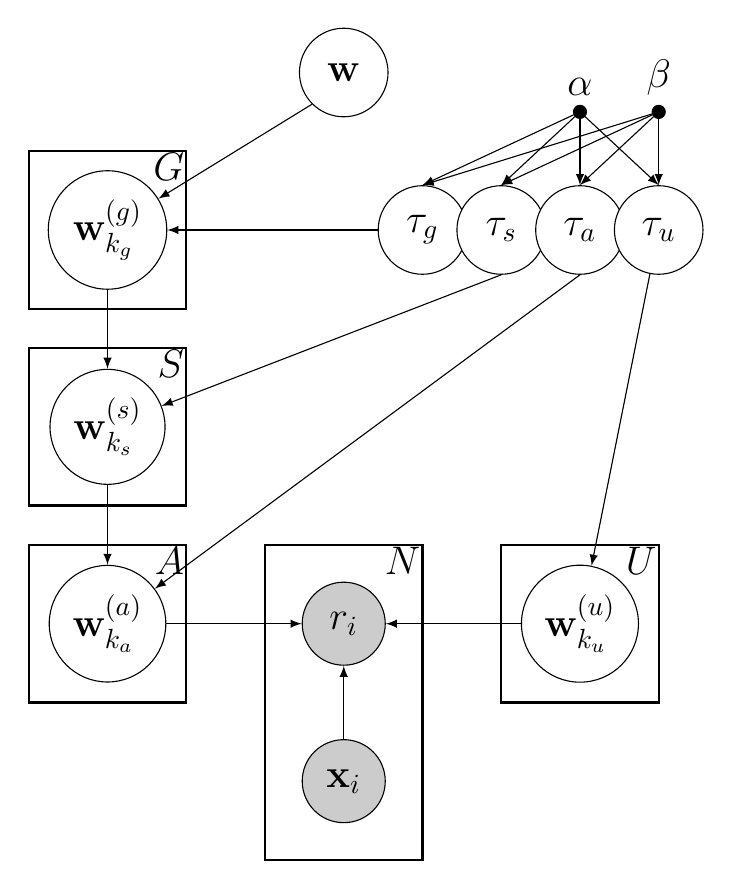
\begin{tikzpicture}[scale=1,,font=\Large,darkstyle/.style={circle,draw,fill=white!40,minimum size=32}]
		\tikzstyle{obsnode}=[circle,draw,fill=gray!40,minimum size=30]
		\tikzstyle{dot}=[circle,draw,fill=black,scale=0.5		]
		\tikzstyle{plate}=[draw,thick,minimum width=2cm,minimum height=2cm]
				\tikzstyle{plate2}=[draw,thick,minimum width=2cm,minimum height=4cm]
		\tikzstyle{line}=[draw]
		\tikzstyle{arrow}=[draw, -latex ]
		\tikzstyle{level 1}=[sibling distance=50mm]
		\tikzstyle{level 2}=[sibling distance=25mm]
		\tikzstyle{level 3}=[sibling distance=12mm]
		\tikzstyle{level 4}=[sibling distance=6mm]
		\tikzstyle{level 5}=[sibling distance=4mm,level distance=10mm]

\node[darkstyle](w) at(0,0){\textbf{w}} ;
\node[darkstyle](tg) at(1,-2){$\tau_g$} ;
\node[darkstyle](ts) at(2,-2){$\tau_s$} ;
\node[darkstyle](ta) at(3,-2){$\tau_a$} ;
\node[darkstyle](tu) at(4,-2){$\tau_u$} ;
\node[dot,label=above:{$\alpha$} ](alpha) at(3,-0.5){} ;
\node[dot,label=above:{$\beta$} ](beta) at(4,-0.5){} ;
\node[plate] (pg) at (-3,-2){} ;
		\node[darkstyle](g) at (-3,-2){$\textbf{w}^{(g)}_{k_g}$};
		\node[anchor=north east,inner sep=1pt] at (pg.north east){$G$};
		
		\node[plate] (ps) at (-3,-4.5){} ;
				\node[darkstyle](s) at (-3,-4.5){$\textbf{w}^{(s)}_{k_s}$};
		\node[anchor=north east,inner sep=1pt] at (ps.north east){$S$};
				\node[plate] (pa) at (-3,-7){} ;
				\node[darkstyle](a) at (-3,-7){$\textbf{w}^{(a)}_{k_a}$};
		\node[anchor=north east,inner sep=1pt] at (pa.north east){$A$};
					\node[plate] (pu) at (3,-7){} ;
		\node[darkstyle](u) at (3,-7){$\textbf{w}^{(u)}_{k_u}$};
		\node[anchor=north east,inner sep=1pt] at (pu.north east){$U$};
		
		\node[plate2] (p) at (0,-8){} ;
		\node[obsnode](r) at (0,-7){$r_{i}$};
		\node[obsnode](x) at (0,-9){$\x_{i}$};
		\node[anchor=north east,inner sep=1pt] at (p.north east){$N$};
\path[arrow]  (x) -- (r){};
\path[arrow]  (u) -- (r){};
\path[arrow]  (a) -- (r){};
\path[arrow]  (w.south west) -- (g){};
\path[arrow]  (g) -- (s){};
\path[arrow]  (s) -- (a){};
\path[arrow]  (ts.south) -- (s){};
\path[arrow]  (tg) -- (g){};
\path[arrow]  (ta.south) -- (a){};
\path[arrow]  (tu) -- (u){};
\path[arrow]  (alpha) -- (tu.north){};
\path[arrow]  (alpha) -- (ta.north){};
\path[arrow]  (alpha) --(tg.north){};
\path[arrow]  (alpha) -- (ts.north){};
\path[arrow]  (beta) -- (tu.north){};
\path[arrow]  (beta) -- (ta.north){};
\path[arrow]  (beta) -- (tg.north){};
\path[arrow]  (beta) -- (ts.north){};
	
	
		\end{tikzpicture}}
	%\vspace{-0.5cm}
	\end{center}
	\caption{A graphical model representation of the proposed model. Unshaded circles denote unobserved random variables. Shaded circles denote observed random variables. Solid dots denote hyper-parameters. }
	\label{fig:graphical_model}
\end{figure}


\subsection{Variational Inference}
We apply variational inference (or variational Bayes) to approximate the posterior distribution,
$p(\btheta | \mathcal{D}, \mathcal{H} )$,  with some distribution $q(\btheta)$,
by maximizing the (negative) variational free energy given by
$
\mathcal{F} [ q(\btheta) ] \defined \int q(\btheta) \log \frac{p(\mathcal{D}, \btheta | \mathcal{H})}{q(\btheta)} \, \mathrm{d} \btheta
$.
$\mathcal{F}$ serves as a lower bound on the log marginal likelihood, or logarithm of the model evidence. 

\subsubsection{Logistic Bound}
The joint probability in (\ref{eq:joint-likelihood}) includes Gaussian priors which are not conjugate to the likelihood, due to the sigmoid functions appearing in (\ref{eq:likelihood}).
In order to facilitate approximate inference, these sigmoid functions are bounded by a ``squared exponential'' form, which is conjugate to the Gaussian prior. 
The following derivations resemble variational inference for logistic regression as described in more detail in \cite{LogisticBound}.

First, the sigmoid functions appearing in (\ref{eq:joint-likelihood}) are lower-bounded using the logistic bound \cite{VB_Methods}.
Introducing an additional variational parameter $\xi_i$ on each observation $i$ allows the following bound:
\begin{equation}
\begingroup\makeatletter\def\f@size{\fsize}\check@mathfonts
\def\maketag@@@#1{\hbox{\m@th\large\normalfont#1}}%
\begin{aligned}
& \sigma(h_i)^{r_i} \cdot \left[ 1- \sigma(h_i)\right]^{1-r_i} \geq  \sigma(\xi_i) e^{r_ih_i-\frac{1}{2}(h_i+\xi_i)-\lambda_i(h_i^2+\xi_i^2)}
\label{eq:Jordan-Jakkola}
\end{aligned}\endgroup
\end{equation} 
where $h_i \defined \x_i^\top ( \w^{(a)}_{a_i} + \w^{(u)}_{u_i} )$ and
$\lambda_i \defined \frac{1}{2 \xi_i} [ \sigma(\xi_i)-\frac{1}{2} ]$.
Using (\ref{eq:Jordan-Jakkola}), we substitute for the sigmoid functions in $p(\mathcal{D}, \btheta | \mathcal{H})$
to obtain the lower bound $p_{\xi}(\mathcal{D}, \btheta | \mathcal{H})$.
We can apply this bound to the variational free energy:
\[
\mathcal{F}[ q(\btheta)] \geq \mathcal{F}_{\xi}[ q(\btheta)] \defined  \int q(\btheta) \log \frac{p_{\xi}(\mathcal{D}, \btheta  | \mathcal{H})}{q(\btheta)} \, \mathrm{d} \btheta \ .
\]
The analytically tractable $\mathcal{F}_{\xi}[ q(\btheta)]$ is used as our optimization objective with respect to our approximate posterior distribution $q(\btheta)$. 


\subsubsection{Update Equations}
Variational inference is achieved by restricting the approximation distribution $q(\btheta)$ to
the family of distributions that factor over the parameters in $\btheta$. With a slight notation overloading for $q$ we have  
\begin{equation}
\begingroup\makeatletter\def\f@size{\fsize}\check@mathfonts
\def\maketag@@@#1{\hbox{\m@th\large\normalfont#1}}%
\begin{aligned}
q(\btheta)= & \prod_{k_u=1}^U q(\w_{k_u}^{(u)}) \cdot \prod_{k_a=1}^A q(\w_{k_a}^{(a)}) \cdot \prod_{k_s=1}^S q(\w_{k_s}^{(s)}) \cdot \prod_{k_g=1}^G q(\w_{k_g}^{(g)}) \\
& \cdot q(\w) \cdot q(\tau_u) \cdot q(\tau_a) \cdot q(\tau_s) \cdot q(\tau_g) \cdot q(\tau_w), 
\label{eq:factorized_q}
\end{aligned}\endgroup
\end{equation} 
where $q$ denotes a different distribution function for each parameter in $\btheta$.
%Overall we have $U+G+S+A+1$ parameter vectors (the $\w$'s) and $5$ precision parameters (the $\tau$'s).

Optimization of $\mathcal{F}_{\xi}$ follows using coordinate ascent in the function space of the variational distributions. 
Namely, we compute functional derivatives $\partial\mathcal{F}_{\xi} / \partial q $ with respect to each
distribution $q$ in (\ref{eq:factorized_q}). 
Equating the derivatives to zero, together with a Lagrange multiplier constraint to make $q$ integrate
to 1 (a distribution function), we get the update equations for each $q$ in (\ref{eq:factorized_q}). At each iteration, the optimization process alternates through parameters, applying each update equation in turn. 
Each such update increases the objective $\mathcal{F}_{\xi}$, thus increasing $\mathcal{F}$. We continue to iterate until convergence.
Owing to the analytical form of $\mathcal{F}_{\xi}$ and the factorization assumption on the approximation distribution $q$, each component of $q$ turns out to be Gaussian distributed, in the case of the weight parameters, or Gamma distributed, in the case of the precision parameters.
Thus, in the following we describe the update step of each component of $q$ in terms of its canonical parameters.


\paragraph{Update for user parameters}
\noindent For each user $k_u=1\dots U$ we approximate the posterior of $\w^{(u)}_{k_u}$ with a Gaussian distribution 
\begin{equation}
\begingroup\makeatletter\def\f@size{\fsize}\check@mathfonts
\def\maketag@@@#1{\hbox{\m@th\large\normalfont#1}}%
\begin{aligned}
& q(\w^{(u)}_{k_u})=\mathcal{N}\left(\textbf{w}^{(u)}_{k_u}; \bmu^{(u)}_{k_u}, \bSigma^{(u)}_{k_u} \right), 
\label{eq:q_u}
\end{aligned}\endgroup
\end{equation} 
\begin{equation}
\begingroup\makeatletter\def\f@size{\fsize}\check@mathfonts
\def\maketag@@@#1{\hbox{\m@th\large\normalfont#1}}%
\begin{aligned}
\bSigma^{(u)}_{k_u} = &\left[\tau_u \I +\sum_{i=1}^N \mathbb{I}\left[u_i=k_u\right]2\lambda_i \cdot \x_i\x_i^\top  \right]^{-1} \\ \nonumber
\bmu^{(u)}_{k_u}= & \bSigma^{(u)}_{k_u} \cdot\left[\sum_{i=1}^N \mathbb{I}\left[u_i=k_u\right]   \left(r_i-\frac{1}{2} - 2\lambda_i \x_i^\top \langle \textbf{w}^{(a)}_{a_i} \rangle \right) \x_i \right],
\end{aligned}\endgroup
\end{equation} 
where $\mathbb{I}\left[ \cdot \right]$ is an indicator function. 
The angular brackets are used to denote an expectation over $q(\btheta)$ i.e., $\langle \w^{(a)}_{a_i}\rangle = \mathbb{E}_{q(\btheta)} [ \w^{(a)}_{a_i}  ]$
\GL{actually, the expectation here is over all $\btheta$ except for $\w^{(u)}_{k_u}$. I'm not so sure this distinction is important though?}
\todo{It's fine; we can include $\w^{(u)}_{k_u}$ in the expectation, as it's not in the argument of $\mathbb{E}_{q(\btheta)} [ \w^{(a)}_{a_i}  ]$ and will just integrate out to one.}\GL{cool lets leave it as is} \noam{Agree!}


\paragraph{Update for artist parameters}
\noindent For each artist $k_a=1 \dots A$ we approximate the posterior of $\w^{(a)}_{k_a}$ with a Gaussian distribution
\begin{equation}
\begingroup\makeatletter\def\f@size{\fsize}\check@mathfonts
\def\maketag@@@#1{\hbox{\m@th\large\normalfont#1}}%
\begin{aligned}
& q(\w^{(a)}_{k_a})=\mathcal{N}\left(\w^{(a)}_{k_a}; \bmu^{(a)}_{k_a}, \bSigma^{(a)}_{k_a} \right), 
\label{eq:q_a}
\end{aligned}\endgroup
\end{equation} 
\begin{equation}
\begingroup\makeatletter\def\f@size{\fsize}\check@mathfonts
\def\maketag@@@#1{\hbox{\m@th\large\normalfont#1}}%
\begin{aligned}
& \bSigma^{(a)}_{k_a}  =\left[\tau_a \cdot \I+\sum_{i=1}^N \mathbb{I}\left[a_i=k_a\right]2\lambda_i \cdot \x_i\x_i^\top  \right]^{-1}, \\
& \bmu^{(a)}_{k_a} = \bSigma^{(a)}_{k_a} \cdot \Bigg[ \tau_a \langle \w^{(s)}_{\parent(k_a)}\rangle +\\
 &\qquad{}\qquad{}\qquad{} \sum_{i=1}^N \mathbb{I}\left[a_i=k_a\right] \left(r_i-\frac{1}{2} - 2\lambda_i \textbf{x}_i^\top \langle\w^{(u)}_{u_i}\rangle \right) \x_i \Bigg]. \nonumber
\end{aligned}\endgroup
\end{equation}

\newpage
\paragraph{Update for sub-genre parameters}
\noindent For each sub-genre $k_s=1\dots S$ we approximate the posterior of $\w^{(s)}_{k_s}$ with a Gaussian distribution
\begin{equation}
\begingroup\makeatletter\def\f@size{\fsize}\check@mathfonts
\def\maketag@@@#1{\hbox{\m@th\large\normalfont#1}}%
\begin{aligned}
q(\w^{(s)}_{k_s})=\mathcal{N}\left(\w^{(s)}_{k_s}; \bmu^{(s)}_{k_s}, \bSigma^{(s)}_{k_s} \right),
\end{aligned}\endgroup
\end{equation} 
\begin{equation}
\begingroup\makeatletter\def\f@size{\fsize}\check@mathfonts
\def\maketag@@@#1{\hbox{\m@th\large\normalfont#1}}%
\begin{aligned}
\bSigma^{(s)}_{k_s} =&\left(\tau_s+|\mathcal{C}_{k_s}|\tau_a\right)^{-1}\cdot  \I , \nonumber \\
\bmu^{(s)}_{k_s} = &\bSigma^{(s)}_{k_s} \cdot\left[\tau_s \langle \w^{(g)}_{\parent(k_s)}\rangle+\tau_a\sum_{k_a \in \mathcal{C}_{k_s}} \langle \w^{(a)}_{k_a} \rangle \right] ,
\end{aligned}\endgroup
\end{equation}
where $\mathcal{C}_{k_s}=\children(k_s)$ is the set of artists in sub-genre $k_s$.

\paragraph{Update for genre parameters}
\noindent For each genre $k_g=1\dots G$ we approximate the posterior of $\w^{(g)}_{k_g}$ with a Gaussian distribution
\begin{equation}
\begingroup\makeatletter\def\f@size{\fsize}\check@mathfonts
\def\maketag@@@#1{\hbox{\m@th\large\normalfont#1}}%
\begin{aligned}
q(\w^{(g)}_{k_g})=\mathcal{N}\left(\w^{(g)}_{k_g}; \bmu^{(g)}_{k_g}, \bSigma^{(g)}_{k_g} \right),
\end{aligned}\endgroup
\end{equation} 
\begin{equation}
\begingroup\makeatletter\def\f@size{\fsize}\check@mathfonts
\def\maketag@@@#1{\hbox{\m@th\large\normalfont#1}}%
\begin{aligned}
\bSigma^{(g)}_{k_g} = & \left(\tau_g+|\mathcal{C}_{k_g}|\tau_s\right)^{-1} \cdot  \textbf{I}, \nonumber \\
\bmu^{(g)}_{k_g}=&\bSigma^{(g)}_k \cdot\left[\tau_g \langle \w \rangle  +\tau_s\sum_{k_s\in \mathcal{C}_{k_g}}\langle \w^{(s)}_{k_s}\rangle \right],
\end{aligned}\endgroup
\end{equation}
where $\mathcal{C}_{k_g}=\children(k_g)$ is the set of sub-genres for genre $k_g$.

\paragraph{Update for global parameters}
\noindent We approximate the posterior over $\w$ with a Gaussian distribution  
\begin{equation}
\begingroup\makeatletter\def\f@size{\fsize}\check@mathfonts
\def\maketag@@@#1{\hbox{\m@th\large\normalfont#1}}%
\begin{aligned}
& q(\w)=\mathcal{N}\left(\w ; \bmu, \bSigma \right), 
\label{eq:q_w}
\end{aligned}\endgroup
\end{equation} 
\begin{equation}
\begingroup\makeatletter\def\f@size{\fsize}\check@mathfonts
\def\maketag@@@#1{\hbox{\m@th\large\normalfont#1}}%
\begin{aligned}
\bSigma=\left(\tau_w+ \tau_g \cdot G \right)^{-1} \cdot \I \quad \text{and} \quad \bmu=\Sigma\cdot\left[\tau_g\sum_{k_g=1}^{G} \langle \w^{(g)}_{k_g} \rangle \right]. \nonumber
\end{aligned}\endgroup
\end{equation}

\paragraph{Update for the precision parameters}
\noindent The model includes 5 precision parameters: $\tau_u, \tau_a, \tau_s, \tau_g, \tau_w$. Each is approximated with a Gamma distribution. For the sake of brevity we will only provide the update for $\tau_u$. We approximate its posterior with $q(\tau_u)= \mathcal{G}(\tau_u\mid \alpha_u, \beta_u)$, where $\alpha_u=\alpha+\frac{d \cdot U}{2}$ is the shape and $\beta_u=\beta+\frac{1}{2}\sum_{k_u=1}^U\langle \left(\w^{(u)}_{k_u}\right)^{\top} \w^{(u)}_{k_u}\rangle$ is the rate. \GL{This is the one part I did not derive myself. Has anyone verified this?} \noam{I did this very quickly. we can derive it again together. It's no difficult.}\GL{Noam and I verified this expression}


\paragraph{Update for variational parameters}
\noindent The variational parameters $\xi_1\dots \xi_N$ in $\mathcal{F}_{\xi}$ are chosen to maximize $\mathcal{F}_{\xi}$ such that the bound on $\mathcal{F}$ is tight. This is achieved by setting 
$\xi_i= \sqrt{ \langle  \left(\x_i^\top \left( \w^{(a)}_{a_i}+\w^{(u)}_{u_i} \right) \right)^2 \rangle}$. We refer the reader to Bishop \cite{Bishop} for a deeper discussion.

\subsection{Prediction and Ranking}
At run time, given a seed artist $a^*$ and a user $u^*$, our model  computes the probability of a positive outcome for each context vector $\x_1 \dots \x_M$ corresponding to $M$ possible tracks. This probability is given by:

\begin{equation}
\begingroup\makeatletter\def\f@size{\fsize}\check@mathfonts
\def\maketag@@@#1{\hbox{\m@th\large\normalfont#1}}%
\begin{aligned}
\hat{r}_m & \defined p(r_m=1 \mid \x_m,\mathcal{D},  \mathcal{H}) \\
& \approx \int \sigma(h_m)q(\btheta)d \btheta  
 = \int \sigma(h_m) \mathcal{N} \left(h_m \mid \mu_m, \sigma_m^2 \right) d h_m
%& \text{where} \qquad h_m=\x_m^\top \left(\w_u^{(u)}+\w_a^{(a)} \right)
\label{eq:prediction}
\end{aligned}\endgroup
\end{equation}
where the random variable $h_m$ has a Gaussian distribution: %	 (see \cite{Bishop} 4.5.2):  
\begin{equation}
\begingroup\makeatletter\def\f@size{7}\check@mathfonts
\def\maketag@@@#1{\hbox{\m@th\large\normalfont#1}}%
\begin{aligned}
& h_m=\x_m^\top \left(\w_{u^*}^{(u)}+\w_{a^*}^{(a)} \right) \sim \mathcal{N} \left(h_m \mid \mu_m, \sigma_m^2 \right), \\
& \mu_m \defined \langle \x_m^\top \left(\w_{u^*}^{(u)}+\w_{a^*}^{(a)} \right) \rangle,
 \quad \sigma_m^2 \defined \langle \left( \x_m^\top \left(\w_{u^*}^{(u)}+\w_{a^*}^{(a)} \right) - \mu_m \right)^2 \rangle. \nonumber
\end{aligned}\endgroup
\end{equation}
Finally, the integral in (\ref{eq:prediction}) is approximated following MacKay \cite{MacKay92} using
\begin{equation}
\begingroup\makeatletter\def\f@size{\fsize}\check@mathfonts
\def\maketag@@@#1{\hbox{\m@th\large\normalfont#1}}%
\begin{aligned}
\int \sigma(h_m) \mathcal{N} \left(h_m \mid \mu_m, \sigma_m^2 \right) d h_m \approx \sigma \left( \mu_m / \sqrt{1+\pi\sigma_m^2/8}\right).
\end{aligned}\endgroup
\label{eq:PredictionApproximation}
\end{equation}

%\GL{Not sure the below passage is still relevant. I previously added it to adress ulrich's comment of having a way to index the model in the notation. Since then the part applying this has been removed from the section on AuC. WDYT?}
%In the experiment section below we consider several variants of the approach as comparison baselines. Essentially each of these setups considers a subset $\phi$ of the full parameter set $\btheta$. As such we denote the prediction such a model as $p_\phi(r_m=1 \mid \x_m,\mathcal{D},  \mathcal{H})$. For example, the non-personalized partial two-level (root and genre) hierarchy model only learns the parameter subset $\phi_1=\{ \{ \w_{k_g}^{(g)} \}_{k_g=1}^G, \w, \tau_g, \tau_w \}$. The probability of a positive outcome under this model is indexed by this parameter set and denoted $p_{\phi_1}(r_m=1 \mid \x_m,\mathcal{D},  \mathcal{H})$.

%\vspace{-2mm}    
\section{Features for Encoding Context}
\label{sec:Features}
	%\GL{'Contextual features' does not mean anything to me I prefer 'Useful Features for Encoding Context'}
%\GL{In writing this section I believe we should speak to the potential of what is possible with the various sources of information that we have in our possession rather than what we actually used (a subset).THis is similar to our inclusion of the gamma priors over the precision params. This was my approach in rewriting this section.}
The model as described in the previous section makes no assumptions on the nature of the contextual features beyond the fact that they encode relevant information for choosing the next track to be added to the playlist.  
Since the main contribution of this paper is in the definition of the model and corresponding learning algorithm, our efforts to find the best features for the application of playlist generation are by no means exhaustive. 
However, in this section we offer some insights into the types of features used by the algorithm.


%Each of the feature groups above is used to compute pairwise similarities comparing a candidate track to be added to the list with the previous tracks already in the playlist as well as with similarities to the seed artist. 
In general, the features encode different types of similarities or relations  comparing a candidate track and its corresponding artist to be added to the playlist with tracks (and artists) previously selected as well as with the seed artist. In cases where specific similarities are not applicable we apply zero-imputation.
%In our practice the number of features, denoted $d$ below, is on the order of 10-20, including a fixed feature always set to 1 to generalize the approach to include ``biases". 
We include a fixed feature always set to 1 to account for ``biases'' (intercept). 
We divide the features into four groups categorized according to the type of signal employed in their calculation:


\noindent{\bf Acoustic Audio Features (AAF)} -
These features capture acoustic similarity between musical artists by learning a Gaussian Mixture Model (GMM) over mel frequency cepstrum coefficients (MFCC) of an artist's audio samples. The approach follows the model of~\cite{ReynoldsQD00} for speaker identification: 
Let $\mathcal{D}_a=\left\{\mathbf{z}_i \in \mathbb{R}^\ell\right\}$ denote the mel frequency cepstrum coefficients (MFCC) of audio samples from a particular artist $a$. 
%To compute the audio features $\mathbf{z}_i$, we compute the mel frequency cepstrum coefficients (MFCC). 
%First, we find a 256 dimensional universal background model (UBM) for all artists. We denote by $\phi$ the UBM parameters. 
Let $\hat{\phi}_a=\argmax_{\phi} \prod_{\mathbf{z}_i\in\mathcal{D}_a} p\left(\mathbf{z}_i\mid\phi\right)$ denote the maximum likelihood parameter setting of the GMM for a particular artist $a$. The audio similarity between two artists $a_1$ and $a_2$ is then given by \begin{equation}\textsc{KL}\left[ p\left(\mathbf{z_*}\mid\hat{\phi}_{a_1}\right) \quad \middle| \middle| \quad  p\left(\mathbf{z_*} \mid \hat{\phi}_{a_2}\right)\right
],\end{equation} the Kullback Liebler divergence between the two corresponding distributions.
Track to track similarities are computed in a similar fashion by considering GMMs over audio samples from individual tracks.  

\noindent{\bf Usage Features (UF)} -
Following \cite{xbox-www} we learn a low-rank factorization of the matrix $\mathcal{R}$,
 where $r_{i,j}$ the element on the $i$-th row and $j$-th column denotes the binary rating given to the $j$-th artist in the catalog by the $i$-th user of the system. This formulation is parameterized by a $k$-dimensional vector for each user and artist appearing in the training data. More precisely, the user vectors $\left\{\mathbf{u}_i\right\}_{i=1}^{|U|}$ and artist vectors $\left\{\mathbf{a}_j\right\}_{j=1}^{|A|}$, collectively denoted $\phi_u$ are chosen to optimize the Bayesian model $p(\mathcal{D}_u,\phi_u)$ (Equation (5) in \cite{xbox-www}) over the training dataset containing binary interactions between users and artists, denoted $\mathcal{D}_u$.  The similarity between two artists $a_1$ and $a_2$ is then given by $\sigma \left(\mathbf{a}_{a_1}^\top\mathbf{a}_{a_2}\right)$, where $\sigma$ denotes the sigmoid function. A similar treatment can be applied to a matrix of user-track interaction and used to derive similarities between tracks.

\noindent{\bf Meta-Data Features (MDF)} -
Meta-Data features are based on the semantic tags associated with different tracks and artists in Microsoft's catalog~(e.g. ``easy-listening'', ``upbeat'', ``90's''). Each artist $j$ in the catalog is  encoded as a vector $\mathbf{b}_j \in \left\{0,1\right\}^{|V|}$, where $V$ denotes the set of  possible binary semantic tags. These vectors are generally sparse, as each artist corresponds to only a small number of semantic tags.  The similarity between two artists $a_1$ and $a_2$ is then given by the cosine similarity: 
\begin{equation}\frac{\mathbf{b}_{a_1}^\top\mathbf{b}_{a_2}}{\parallel\mathbf{b}_{a_1}\parallel\parallel\mathbf{b}_{a_2}\parallel}
\end{equation}
Track to track similarity is computed by using sparse vectors representing tracks.

\noindent{\bf Popularity Features (PF)} -
Popularity is a measure of the prevalence of a track or artist in the dataset.
Popularity is used to compute unary features representing the popularity of a candidate track and its artist. For a particular artist $a_1$ such a feature is computed $\textsc{pop}_{a1}=\frac{\#\left(a_1\right)}{|\mathcal{D}_u|}$, where $\#\left(a_1\right)$ denotes the number of users who consumed a track by artist $a_1$  in the training corpus $\mathcal{D}_u$. Pairwise popularity features are computed relating the popularity of the candidate track and its artist to the popularity of the seed artist and previous tracks. The relative popularity of artists $a_1$ and $a_2$ can be computed as $\frac{\textsc{pop}_{a2}}{\textsc{pop}_{a1}}$. Track to track and track to artist relative popularity are computed similarly.


%The above features are computed for the various signal sources, different taxonomy level (i.e. artist or track) and different aggregation levels (e.g. averaged over all previous tracks vs only last track) allows for many features. Then, forward feature selection is performed in order to remove redundant features according to the prediction task at hand.





%
%We base our features on three types of resources. The first one is the audio itself. The Audio Based Similarity (ABS) system maps audio tracks to a vector space. Specifically, for each track we extract 12 MFCCs augmented by delta and delta-delta coefficients to form a frame representation feature vector of dimensionality 36. We use a frame size of 2048 with half overlapping frames \SBE{perhaps translate to stride?}. Then, we learn a background distribution from a subset of the entire dataset. To this end, a background GMM with 256 components is trained by applying Expectation Maximization (EM) \cite{ReynoldsQD00}. Given a set of MFCCs features that are extracted from a specific track, we first apply MAP adaptation \cite{ReynoldsQD00}, where the background GMM distribution is taken as a prior. The final representation is determined from the adapted GMM concatenated means. Therefore, the final representation for each audio track is a 9216 dimensional vector. Using ABS we extract artist to artist, $a2a_{ABS}$, and track to track similarity, $t2t_{ABS}$. These features perceive the audio similarity, but they lack semantics such as popularity and origin. The second resource is the usage we collect from the groove client. Using matrix factorization \SBE{Ref RecoMF?} we extract $a2a_{MF}$ and $t2t_{MF}$ similarity based on usage patterns. From the usage we also compute the track popularity $t_{pop}$ and artist popularity $a_{pop}$. In addition, from manually curated meta-data on artist's genres, we compute genre similarity, $a2a_{g}$, between artists by measuring the genre distance between the artists \SBE{Unclear how we compute this, what is genre distance? Is this Jaccard on the label set?}. 
%
%With these three feature types we provide features for computing the music similarity of tracks from both aspects, the audio content of the track and the social-usage context. 
%
%\begin{table}[h]
%\begin{center}
%\begin{tabular}{|c|c|c|c|}
% \hline
% \diaghead{\theadfont Diag ColumnmnHead II}%
%{Features}{Resource type}&
%\thead{Audio}&\thead{Usage}&\thead{Content}\\
% \hline
% Track to track similarity & \checkmark & \checkmark & \\ 
% \hline
% Artist to artist similarity & \checkmark & \checkmark & \checkmark\\ 
% \hline
% Track popularity & & \checkmark & \\ 
% \hline
% Artist popularity & & \checkmark & \\ 
% \hline
%\end{tabular}
%    \caption{This table shows features we compute from each of the three resources.}
%\end{center}
%\end{table}
%
%To summarize, our feature vector $\x$ is composed of the set of features $\{a2a_{ABS},t2t_{ABS},a2a_{MF},t2t_{MF},a2a_{g},t_{pop},a_{pop}\}$ computed on the context seed artist, current track and candidate track. \SBE{Need to verify that this is the complete feature set and elaborate on relation of features to state}
%

%\vspace{-2mm}	
\newpage
\section{Evaluation}
\label{sec:experiments}
    %!TEX root = RadioPaper_Main.tex
The following section describes the evaluation procedure applied to the proposed algorithm. 
%Results in this section are based on the predicted values $\hat{r}_m$ from (\ref{eq:prediction}), without applying any heuristics.
%For the results, all tracks are considered and picked exactly according to the ranking induced by $\hat{r}_m$ \footnote{\todo{
%We may have to add a footnote that in a production system, there might be additional interleaving and small heuristics, which of course
%we can't explain here. It's both outside the scope of the paper, and the secret in the sauce. Or something like that.
%}}.
%We first provide evidence that personalization is essential to quality in our learning problem. Next we illustrate the importance of different features we used. Finally, we show how our model handles well the ``cold start" problem.

\subsection{Datasets}
As explained in Section~\ref{sec:playlist_is_classification}, the model in this paper treats playlist generation
as a classification problem, for which the parameters can be
learned from examples, judiciously labeled through a variety of approaches.
The  two datasets  used for the evaluations exemplify different approaches to the construction of the training data:

\noindent{\bf Groove Music Dataset}
is a proprietary dataset of user preferences that was collected anonymously from Microsoft's Groove music service.
It contains 334,120 users, 472,908 tracks from 45,239 artists categorized into 100 sub-genres from 17 genres. Positive labels
are assigned to tracks in a user's listening history that were heard to completion. Negative labels are assigned to tracks that were skipped in mid-play by the user.

\noindent{\bf 30Music Dataset}
is a publicly available dataset of user playlists \cite{DBLP:conf/recsys/TurrinQCPC15}. Tracks in this dataset were intersected with Groove's catalog in order to enable feature generation (i.e. audio and content features). The resulting dataset contains 14,185 users, 252,424 tracks from 63,314 artists categorized into 99 sub-genres from 17 genres. Positive labels are assigned to tracks appearing in a user's playlist. Since no skip information was available, negatively labeled examples were obtained by uniformly sampling from tracks that did not appear in the user's playlist.
% \end{enumerate}


\subsection{Experimental Setup and Results}
We quantify the quality of the model using the \textit{Area Under Curve} (AUC) metric \cite{AUCRef}. AUC enables quantifying the trade-off between true positives and false positives over a range of threshold configurations. By doing so, AUC captures the overall quality of a particular prediction method.

%More formally, AUC is given by the following expression over threshold $t$:
%%%
%$$
%\mathrm{AUC} = \int_0^1 \mathrm{TPR}(t) \, \mathrm{FPR'}(t) \, d t
%$$
%%%
%where $\mathrm{FPR}(t)$ and $\mathrm{TPR}(t)$ are the True- and False Positive Rates at threshold $t$ respectively. %(TPR and FPR) are:

%\noam{We need to save space, so assume the reader known TPR and FPR.}
%%%
%\begin{align*}
%\mathrm{TPR}(t) & = \frac{1}{|\mathcal{X}_{\mathrm{pos}} |}
%\sum_{\x \in \mathcal{X}_{\mathrm{pos}}} \mathbb{I} \Big[ \widetilde{p}_{\phi}(r = 1 | \x, \mathcal{D}, \mathcal{H} ) \geq t \Big] \\
%\mathrm{FPR}(t) & = \frac{1}{|\mathcal{X}_{\mathrm{neg}} |}
%\sum_{\x \in \mathcal{X}_{\mathrm{neg}}} \mathbb{I} \Big[ \widetilde{p}_{\phi} (r = 1 | \x, \mathcal{D}, \mathcal{H} ) \geq t \Big] \ .
%\end{align*}
%%%
%$\mathcal{X}_{\mathrm{pos}}$ and $\mathcal{X}_{\mathrm{neg}}$ denote the subset of positive and negatively labeled examples, respectively, of an evaluation set with known labels, while $\phi$ indexes a particular subset of parameters, and
%$\widetilde{p}_{\phi} \in [0,1]$ denotes the probability given by (\ref{eq:PredictionApproximation}).
%\todo{the equation below (\ref{eq:prediction})} 
%The following section outlines the models tested.
%\todo{we have to tidy up notation and write TPR in terms of our actual model. I put a tilde over the $p$ to show that it's an
%approximation, but we can choose anything (and define it earlier). We also have to find a clean way to enumerate ``model'' in our
%notation, and allude to it earlier.}
%\GL{To ulrich's comment above: I added a definiton indexed on the parameter subset denoted $\phi$ in my notation in the last paragraph of the prediction sub-section}
%\todo{I removed threshold $\theta$ here and made it a $t$, so as not to overload symbols.}
%
%% $f\left(x\right) \in [0,1]$ denotes the confidence of the learned classifier.
%
%\todo{In (\ref{eq:prediction}) there should be no $\btheta$ in
%$p(r = 1 | \x, \mathcal{D}, \mathcal{H} )$, as we average over the posterior of $\btheta$ / integrate it out.}

%\subsection{Experimental Procedure}

The model was trained on 70\% of the examples and evaluated on the remaining 30\%. \GLw{We may have more results using cross-validation later in the week, so we can claim a stronger experimental setup}
%In what follows, the full model described in this paper is dubbed as {\bf ``Groove''}.
We compare it against several baselines:\\
%For comparison to our fully personalized, four-level (global, genre, sub-genre, artist) semantic hierarchy classification model we considered the following baselines:
%\todo{we have to find a way to enumerate over this (index this) in ``model''. WDYT?}
{\bf Partial Hierarchy} - This baseline (actually three separate baselines, one for each level of the hierarchy)  learns only a subset of the domain taxonomy parameters, corresponding to increasingly coarser levels in the hierarchy than the four levels of the the full model described in Section~\ref{sec:OurModel}. Evaluations are provided at each of the sub-hierarchies: global (no hierarchy), genre (two-level) , and sub-genre (three-level).\\
{\bf Non-Personalized} - A non-personalized version of the Groove model is evaluated by removing the per-user parameters.%Variants of this baseline are evaluated at each level of the taxonomy hierarchy.
\GLw{Added combined model part.. relating different parametrizations to works from the literature}

\noindent{\bf Combined Models} The framework proposed in this work spans a family of models parameterized by $\eta\in\left\{1,2,3,4\right\}$, the number of levels of the hierarchical taxonomy and $\varphi\in\left\{0,1\right\}$, the absence/presence of a personalization component. Viewed this way, we can roughly equate different configurations of these hyper-params with previous approaches proposed in the literature. For instance the full hierarchy, non-personalized ($\eta=4,\varphi=0$) variant of the model roughly corresponds to the approach proposed in \cite{NIPS2012_4609}. Further, the personalized no-hierarchy variant ($\eta=1,\varphi=1$), corresponds to methods that have attempted to combine different similarity signals without taking into account user preferences~\cite{Knees:2006,McFee_multi_similarities}. Finally, a two-level hierarchy with personalization  ($\eta=2,\varphi=1$) is similar in spirit (though not identical in formulation) to methods that explicitly model biases for different genres \cite{Dror2011,Mnih2012}.

\noindent{\bf Non-Personalized Regression} - This baseline is a simplified version of the model where the likelihood is changed to consider a regression problem and the optimization is based on an maximum a posteriori (MAP) solution (instead of variational Bayes). This method also considers the domain taxonomy, but results are provided only considering the full-hierarchy. \noam{Removing this: ``This method considers the domain taxonomy, but is not easily modified to consider sub-hierarchies.'' Never apologize in a paper. Reviews will prey on you! Reviewers do not deserve apologizes. This can be added for regular reader in CAM-ready version. Remember - Never apologize to a reviewer!}
%\GL{Reading through this it occured to me that we completely left out he results for this baseline. I will add them to the figure and add a small line to the analysis to reflect the change} \noam{IMPORTANT!!!!}

%That is, parameters at each level of the semantic hierarchy are learned separately, using the parent level as a prior. This method has no straightforward extension to accommodate personalization


%%%
%We evaluated the above methods for a range of hyper-parameters, but found the results to be largely
%robust to these settings. As such we do not include these results in the presentation below.


%\paragraph{Semantic Hierarchy And Personalization Effects}



\begin{figure*}
\centering
\scalebox{.5}{
\hspace{-5cm}
\subfigure[Groove Music]
{
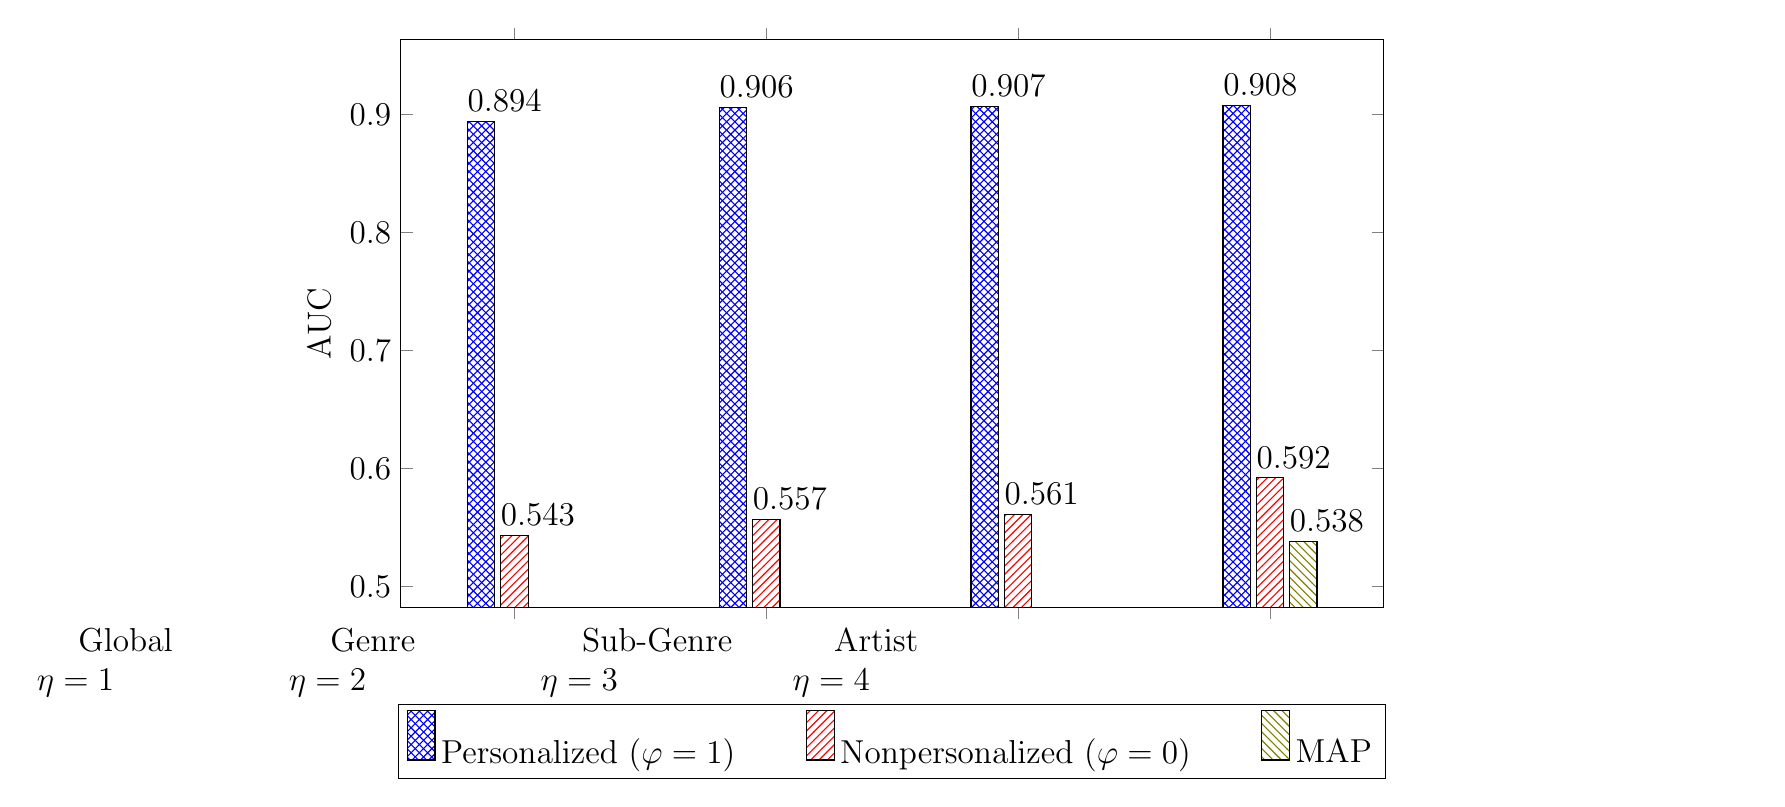
\begin{tikzpicture} 
\begin{axis}[ ybar, enlargelimits=0.15, legend style={font=\large,at={(0.5,-0.17)}, anchor=north,legend columns=-1}, 
/pgf/number format/precision=3,
width=400,height=250,
font=\large,
ylabel={AUC}, 
symbolic x coords={Global,Genre,Sub-Genre,Artist}, 
xtick=data, nodes near coords, nodes near coords align={vertical},xticklabels={\vbox{Global\\ {$\eta=1$}},\vbox{Genre\\ {$\eta=2$}},\vbox{Sub-Genre\\ {$\eta=3$}},\vbox{Artist\\ {$\eta=4$}}},
every node near coord/.append style={xshift=0.3cm}  
 ]
 \addplot[pattern=crosshatch,pattern color=blue]
  %\addplot 
  coordinates {(Global,0.894) (Genre,0.906) (Sub-Genre,0.907)(Artist,0.908)};
 \addplot[pattern=north east lines,pattern color=red ] 
  %\addplot
   coordinates {(Global,0.543) (Genre,0.557) (Sub-Genre,0.561)(Artist,0.592)} ;
   \addplot[pattern=north west lines,pattern color=olive ] coordinates {(Artist,0.538)};
  \legend{Personalized $(\varphi=1)$\qquad{}  ,Nonpersonalized $(\varphi=0)$\qquad{}  ,MAP  }
   \end{axis}
    \end{tikzpicture}

    }
    \hspace{-10cm}
    \subfigure[30Music]
{

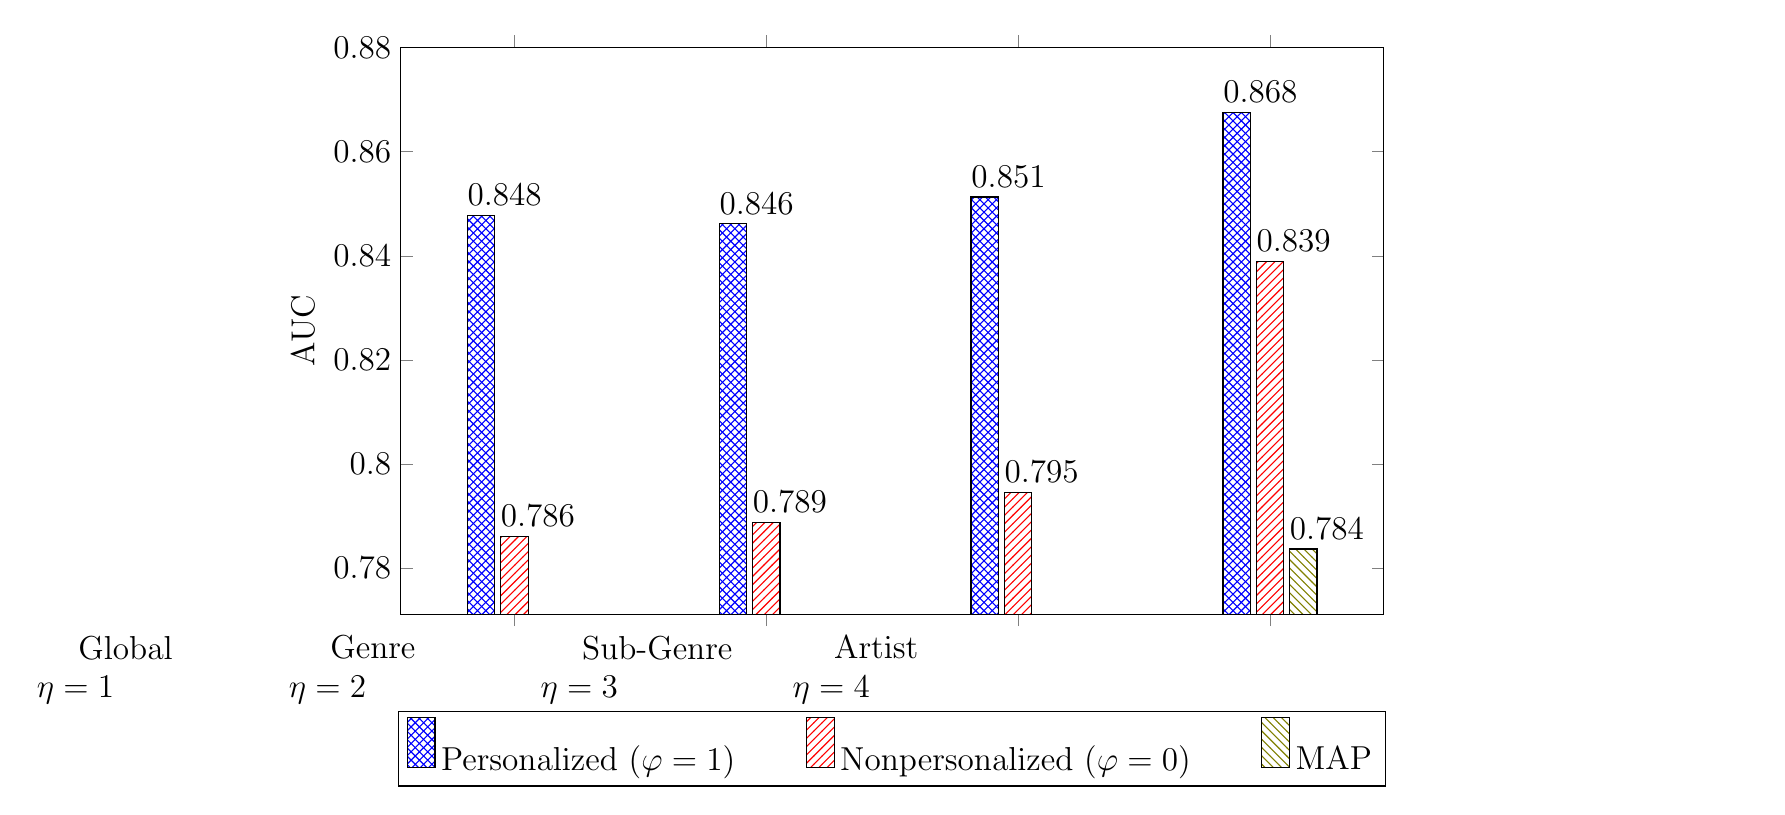
\begin{tikzpicture} 
\begin{axis}[ ybar, enlargelimits=0.15, legend style={font=\large,at={(0.5,-0.17)}, anchor=north,legend columns=-1}, 
/pgf/number format/precision=3,
width=400,height=250,
font=\large,
ylabel={AUC}, 
symbolic x coords={Global,Genre,Sub-Genre,Artist}, 
xtick=data, nodes near coords, nodes near coords align={vertical}, xticklabels={\vbox{Global\\ {$\eta=1$}},\vbox{Genre\\ {$\eta=2$}},\vbox{Sub-Genre\\ {$\eta=3$}},\vbox{Artist\\ {$\eta=4$}}},
every node near coord/.append style={xshift=0.3cm}  
 ]
 \addplot[pattern=crosshatch,pattern color=blue]
  coordinates {(Global,0.847712777) (Genre,0.846150903	) (Sub-Genre,0.851292881)(Artist,0.867522546)};
 \addplot[pattern=north east lines,pattern color=red ] coordinates {(Global,
 %\addplot coordinates {(Global,
0.786095642) (Genre,0.788843283) (Sub-Genre,0.794526999)(Artist,0.838879171)};
\addplot[pattern=north west lines,pattern color=olive ] coordinates {(Artist,0.783697346)};
  \legend{Personalized $(\varphi=1)$\qquad{}  ,Nonpersonalized $(\varphi=0)$\qquad{}  ,MAP  }
   \end{axis}
    \end{tikzpicture}}   } 
    \caption{The effects of personalization and hierarchy on accuracy (as measured by AUC) are illustrated for  (a) the Groove Music dataset (a) the 30Music Dataset. Our framework can be parameterized to generalize several approaches in the literature (see text). }
    \label{fig:MainResultsFig}
\vspace{0.1cm}    
 \end{figure*}
%One important experimental contribution of our work is demonstrating that explicitly modeling the semantic hierarchy associated with the consumer music domain as well as incorporating personalized (i.e. per-user) information can improve the accuracy (as measured by AUC) in the prediction task.
Figure ~\ref{fig:MainResultsFig} depicts the results of the personalized variant of the model vs. the non-personalized baseline, considering gradually increasing partial domain taxonomies along the x-axis of the figure. The \textit{Global}, \textit{Genre}, and \textit{Sub-Genre} labels, denote a one, two, and three level taxonomy, respectively. The \textit{Artist} label denotes the full-hierarchy model shown in Figure~\ref{fig:graphical_model}.

The effect of adding personalization is apparent in both datasets, but more notable in the Groove Music dataset where ``skips'', as opposed to random sampling, are used to define negative labels. This indicates that skipping of tracks has more user-specific dependencies beyond the user's preference for a particular artist or genre.
Also, clearly visible in both datasets is the importance of the hierarchical domain taxonomy: AUC results improve as additional levels of the hierarchy are considered. This effect is more considerable in the 30Music dataset, where we conjecture that the prediction task is based on a ``less personal'' signal. The non-personalized regression baseline performs worse than the proposed model for both datasets. We conjecture this is due to the fact that this model is trained using MAP and does not allow the consideration of the inherent uncertainty at the different levels of the domain taxonomy hierarchy afforded by the Bayesian model.


%\begin{figure}[H]
\centering
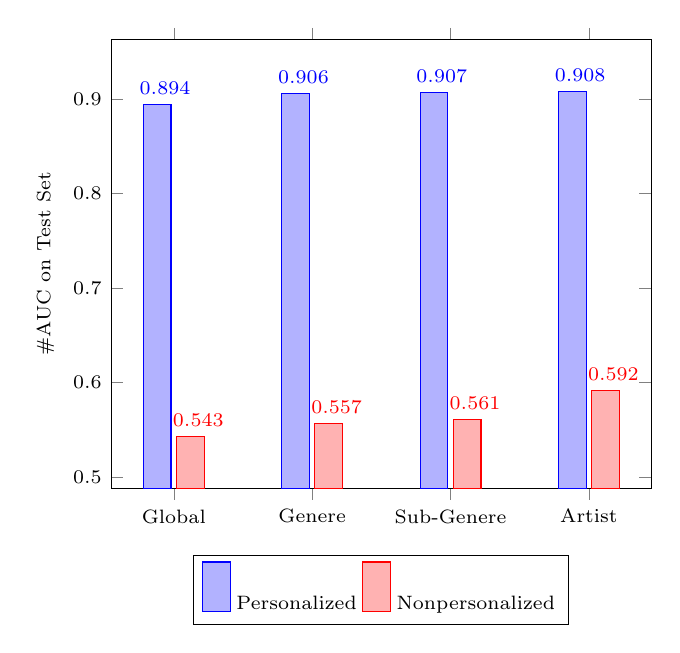
\begin{tikzpicture} 
\begin{axis}[ ybar, enlargelimits=0.15, legend style={at={(0.5,-0.15)}, anchor=north,legend columns=-1}, 
/pgf/number format/precision=5,
font=\scriptsize,
ylabel={\#AUC on Test Set}, 
symbolic x coords={Global,Genere,Sub-Genere,Artist}, 
xtick=data, nodes near coords, nodes near coords align={vertical},
every node near coord/.append style={xshift=0.1cm}  
 ]
 \addplot coordinates {(Global,0.894) (Genere,0.906) (Sub-Genere,0.907)(Artist,0.908)};
 \addplot coordinates {(Global,0.543) (Genere,0.557) (Sub-Genere,0.561)(Artist,0.592)};
  \legend{Personalized,Nonpersonalized}
   \end{axis}
    \end{tikzpicture}
    \caption{Groove Music Dataset}
 \end{figure}
 




%\begin{figure}[H]
\centering

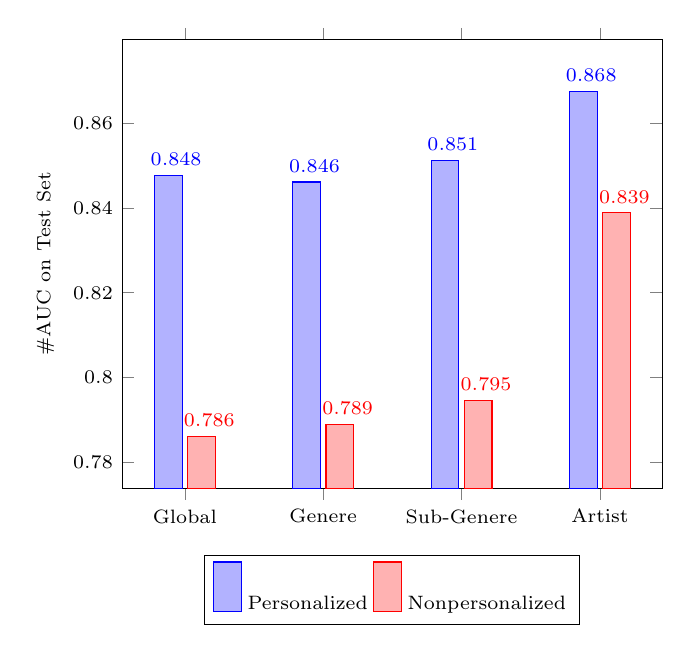
\begin{tikzpicture} 
\begin{axis}[ ybar, enlargelimits=0.15, legend style={at={(0.5,-0.15)}, anchor=north,legend columns=-1}, 
/pgf/number format/precision=3,
font=\scriptsize,
ylabel={\#AUC on Test Set}, 
symbolic x coords={Global,Genere,Sub-Genere,Artist}, 
xtick=data, nodes near coords, nodes near coords align={vertical},
every node near coord/.append style={xshift=0.1cm}  
 ]
 \addplot coordinates {(Global,0.847712777) (Genere,0.846150903	) (Sub-Genere,0.851292881)(Artist,0.867522546)};
 \addplot coordinates {(Global,0.786095642) (Genere,0.788843283) (Sub-Genere,0.794526999)(Artist,0.838879171)};
  \legend{Personalized,Nonpersonalized}
   \end{axis}
    \end{tikzpicture}
    \caption{30 Music Dataset}
 \end{figure}
 



%\paragraph{Effect of Features on Accuracy}
%\begin{figure}

\centering
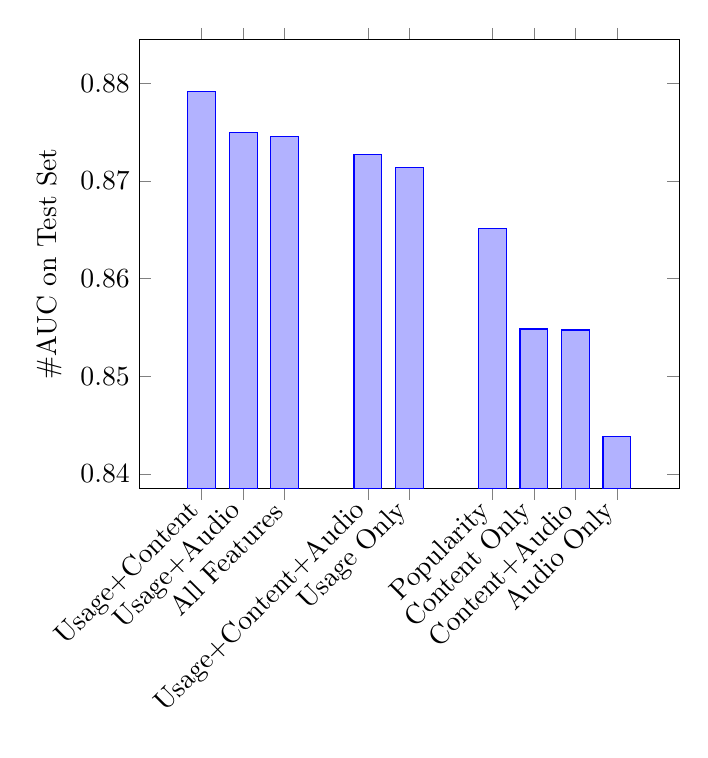
\begin{tikzpicture}
\begin{axis}[ ybar, enlargelimits=0.15, legend style={at={(0.5,-0.15)}, anchor=north,legend columns=-1},
ylabel={\#AUC on Test Set},
symbolic x coords={Usage+Content, Usage+Audio,All Features, ,Usage+Content+Audio, Usage Only, ,Popularity,  Content Only,   Content+Audio,Audio Only},
xtick=data,  nodes near coords align={vertical}, 
x tick label style={rotate=45,anchor=east}
]
 \addplot coordinates {(All Features,0.874533669) (Audio Only,0.843854506)(Content+Audio,0.854736259) (Usage Only, 0.871321339) (Content Only,0.854838861) (Usage+Audio,0.874955404) (Usage+Content,0.879144173)(Popularity,0.865104775)(Usage+Content+Audio,0.872677779)};
 
   \end{axis}
    \end{tikzpicture}
    \caption{Accuracy according to feature group}
    \label{FeaturesFig}
    \end{figure}


\begin{figure}
\scalebox{0.9}{
\begin{tikzpicture}
\begin{axis}[ 
only marks,
ymode=log,xmode=log,
ylabel={Number of Artists},
xlabel={Number of Usage Points}]
\addplot table [x=NumUsagePoints, y=Count, col sep=comma] {histogramOfArtistUsage.csv};


\end{axis}
\end{tikzpicture}}
\caption{A log-log plot of the histogram of usage points for artists in the groove catalog. The large majority of artists have very few observed usage points.}
\label{artistUsageHistFig}
\end{figure}
\input{figs/GenreScatter}

We also considered the contribution of the different feature groups defined in Section~\ref{sec:Features}. To this end we trained the model, using the Groove Music dataset, on each subset of the features separately and evaluated the AUC. Note that for this analysis we used a subset of the data for which no features had missing values. 
%{\bf Usage Features (UF):} These features are derived using collaborative filtering techniques and capture similarity between tracks based on consumption behavior\\
%{\bf Acoustic Audio Features (AAF):} Features based on acoustic audio signals.\\
%{\bf Meta-Data Features (MDF):} Features based on the meta-data features (e.g. "easy-listening", "nineties").\\
%{\bf Popularity Features (PF):} These features simply encode the prevalence of each track in the dataset.\\

Table~\ref{tab:features_AUC} summarizes the  results of this analysis. Using only usage features results in the highest AUC score, followed by popularity, meta-data and acoustic audio features, respectively. Although usage features perform well on their own, we get additional benefits from using other types of features. This is especially relevant when we consider ``cold" artists that have little usage information available. These artists are by far the majority of those appearing in the catalog as can be seen in the histogram (computed over a subset of usage data) shown in Figure~\ref{artistUsageHistFig}.  Furthermore, the importance of usage features in relation to other features varies across the domain taxonomy. Figure~\ref{GenreScatterFig} illustrates this variance. The figure shows that geners such as \textit{Classical} and \textit{Jazz} rely (relatively) much more on audio features and less on usage features than genres such as \textit{Spoken Word} and \textit{Hip~Hop}.


\begin{table}[h!]
\begin{center}
	\begin{tabular}{|c|c|c|c|c|c|}
		\hline
		 & {\bf AAF} & {\bf MDF} & {\bf PF} & {\bf UF} & {\bf All}\\ 
		\hline
		 {\bf AUC} & 0.843  & 0.855 & 0.865 & 0.871 & 0.874\\ 
		\hline
	\end{tabular}
	\vspace{-0.4cm}
\end{center}
\caption{AUC achieved by training only on a subset of features on the Groove Music prediction dataset. Feature groups are defined in Section~\ref{sec:Features}}
\label{tab:features_AUC}
\end{table}



% [NK] - This explanations may belong in the features section but not here.
%In some cases, features were missing due to unavailability of data. Normally, we applied zero imputation whenever a feature is missing for a given context. For this experiment, we discarded examples that had missing values in any of the features.

% [NK] - I don't think this sentence is true.
%Apparent is that AUC values are similary for the various feature groups, indicating low variance. This implies, that the different feature groups contain some redundancy in the information they encode. 

% [NK] - This observation does not contribute to the paper. We need to remove it and remove all the groups that outperm  "All Features":
%This also explains the out-performance of the entire feature set by particular subsets of features, perhaps due to a bias variance tradeoff, i.e, overfitting. This phenomenon was not observed on training-set AUC.






%Further, it is interesting to note that the single feature groups for usage and popularity outperform the single feature groups for content and audio. This is especially noteworthy when considering that audio and content features are significantly more expensive to produce in this domain.


\begin{figure}
\scalebox{0.9}{
\begin{tikzpicture}
\begin{axis}[ legend style={at={(0.7,0.325)}, anchor=north,legend columns=-1},
ylabel={AUC},
xlabel={Cumulative amount of data in training set}]
\addplot table [x=index, y=artist2, col sep=comma] {coldnessData.csv};
\addplot table [x=index, y=user, col sep=comma] {coldnessData.csv};
\legend{Artist,User}

\end{axis}
\end{tikzpicture}}
\caption{A cumulative plot illustrating the effect of Artist/User coldness on test AUC. The AUC is plotted for all Artists/Users with at least $x$ labeled data points in the training set.}
\label{coldnessFig}
\end{figure}
In recommendation systems the cold  user/item problem describes the difficulty of
providing recommendations for users/items with little to no previous interaction with the system. 
Figure \ref{coldnessFig} plots the AUC on the Groove Music dataset as a function of the amount of data available for users and artists, respectively. The plot is cumulative e.g., at value $10$ along the X-axis all users / artists with at most $10$ training examples are considered. AUC levels are significantly lower for cold users but quickly improve as the number of training examples increases. This trend is another indication of the importance of personalized information. In contrast to users, there is almost no change in artists' AUC values per different number of observations, and even artists with zero training examples show high AUC values.
This is enabled due to the models use of the domain taxonomy to mitigate the cold artist problem. %The representation of  other artists in the same genre and sub-genre is used in order to allow accurate prediction for artists that have not been at all observed in the training data. 

%We can see that very ``cold" users have dramatically worse predictions than overall. However, as users with more data become available the accuracy quickly increases. This indicates that ``warmer" users contain predictable patterns that the model is able to harness. Artists, on the other hand, are not as sensitive to ``coldness". This is mainly because the semantic hierarchy utilized in our model allows us to generalize the representation of ``cold" artists using other artists in the same genre and sub-genre. Collectively, these results indicate that we are able to generalize artists by pooling data at lower resolution according to the semantic hierarchy.


\GL{I'm not at all sure about this section, firstly the figure does not translate to black and white and is too small when printed. Furthermore, if artists from the same or similar genres are not close, then what exactly is the claim?} \noam{I think I got an explanation:}
Finally, Figure~\ref{tSNEfig} provides an illustration of artist parameters using a t-SNE embedding \cite{Maaten2008} of artist parameter mean values from the Groove music dataset. 
%The figure shows a rich manifold with mixing between artists of several genres. 
Note that proximity in this plot is determined by similarity in the parameters of the learning model. Namely, it does not necessarily reflect ``musical similarity'', but instead it indicates similarity in the importance of the contextual features. The fact that many artists of the same genre do not cluster together supports the model's underlying assumption from Section~\ref{sec:Introduction} that different considerations needs to be applied when generating their playlists. It also suggests that priors at the genre level alone are too coarse and must be broken down to their sub-genres. 

\begin{figure}[h]
	\vspace{-0.2cm}
	\scalebox{0.3}{
		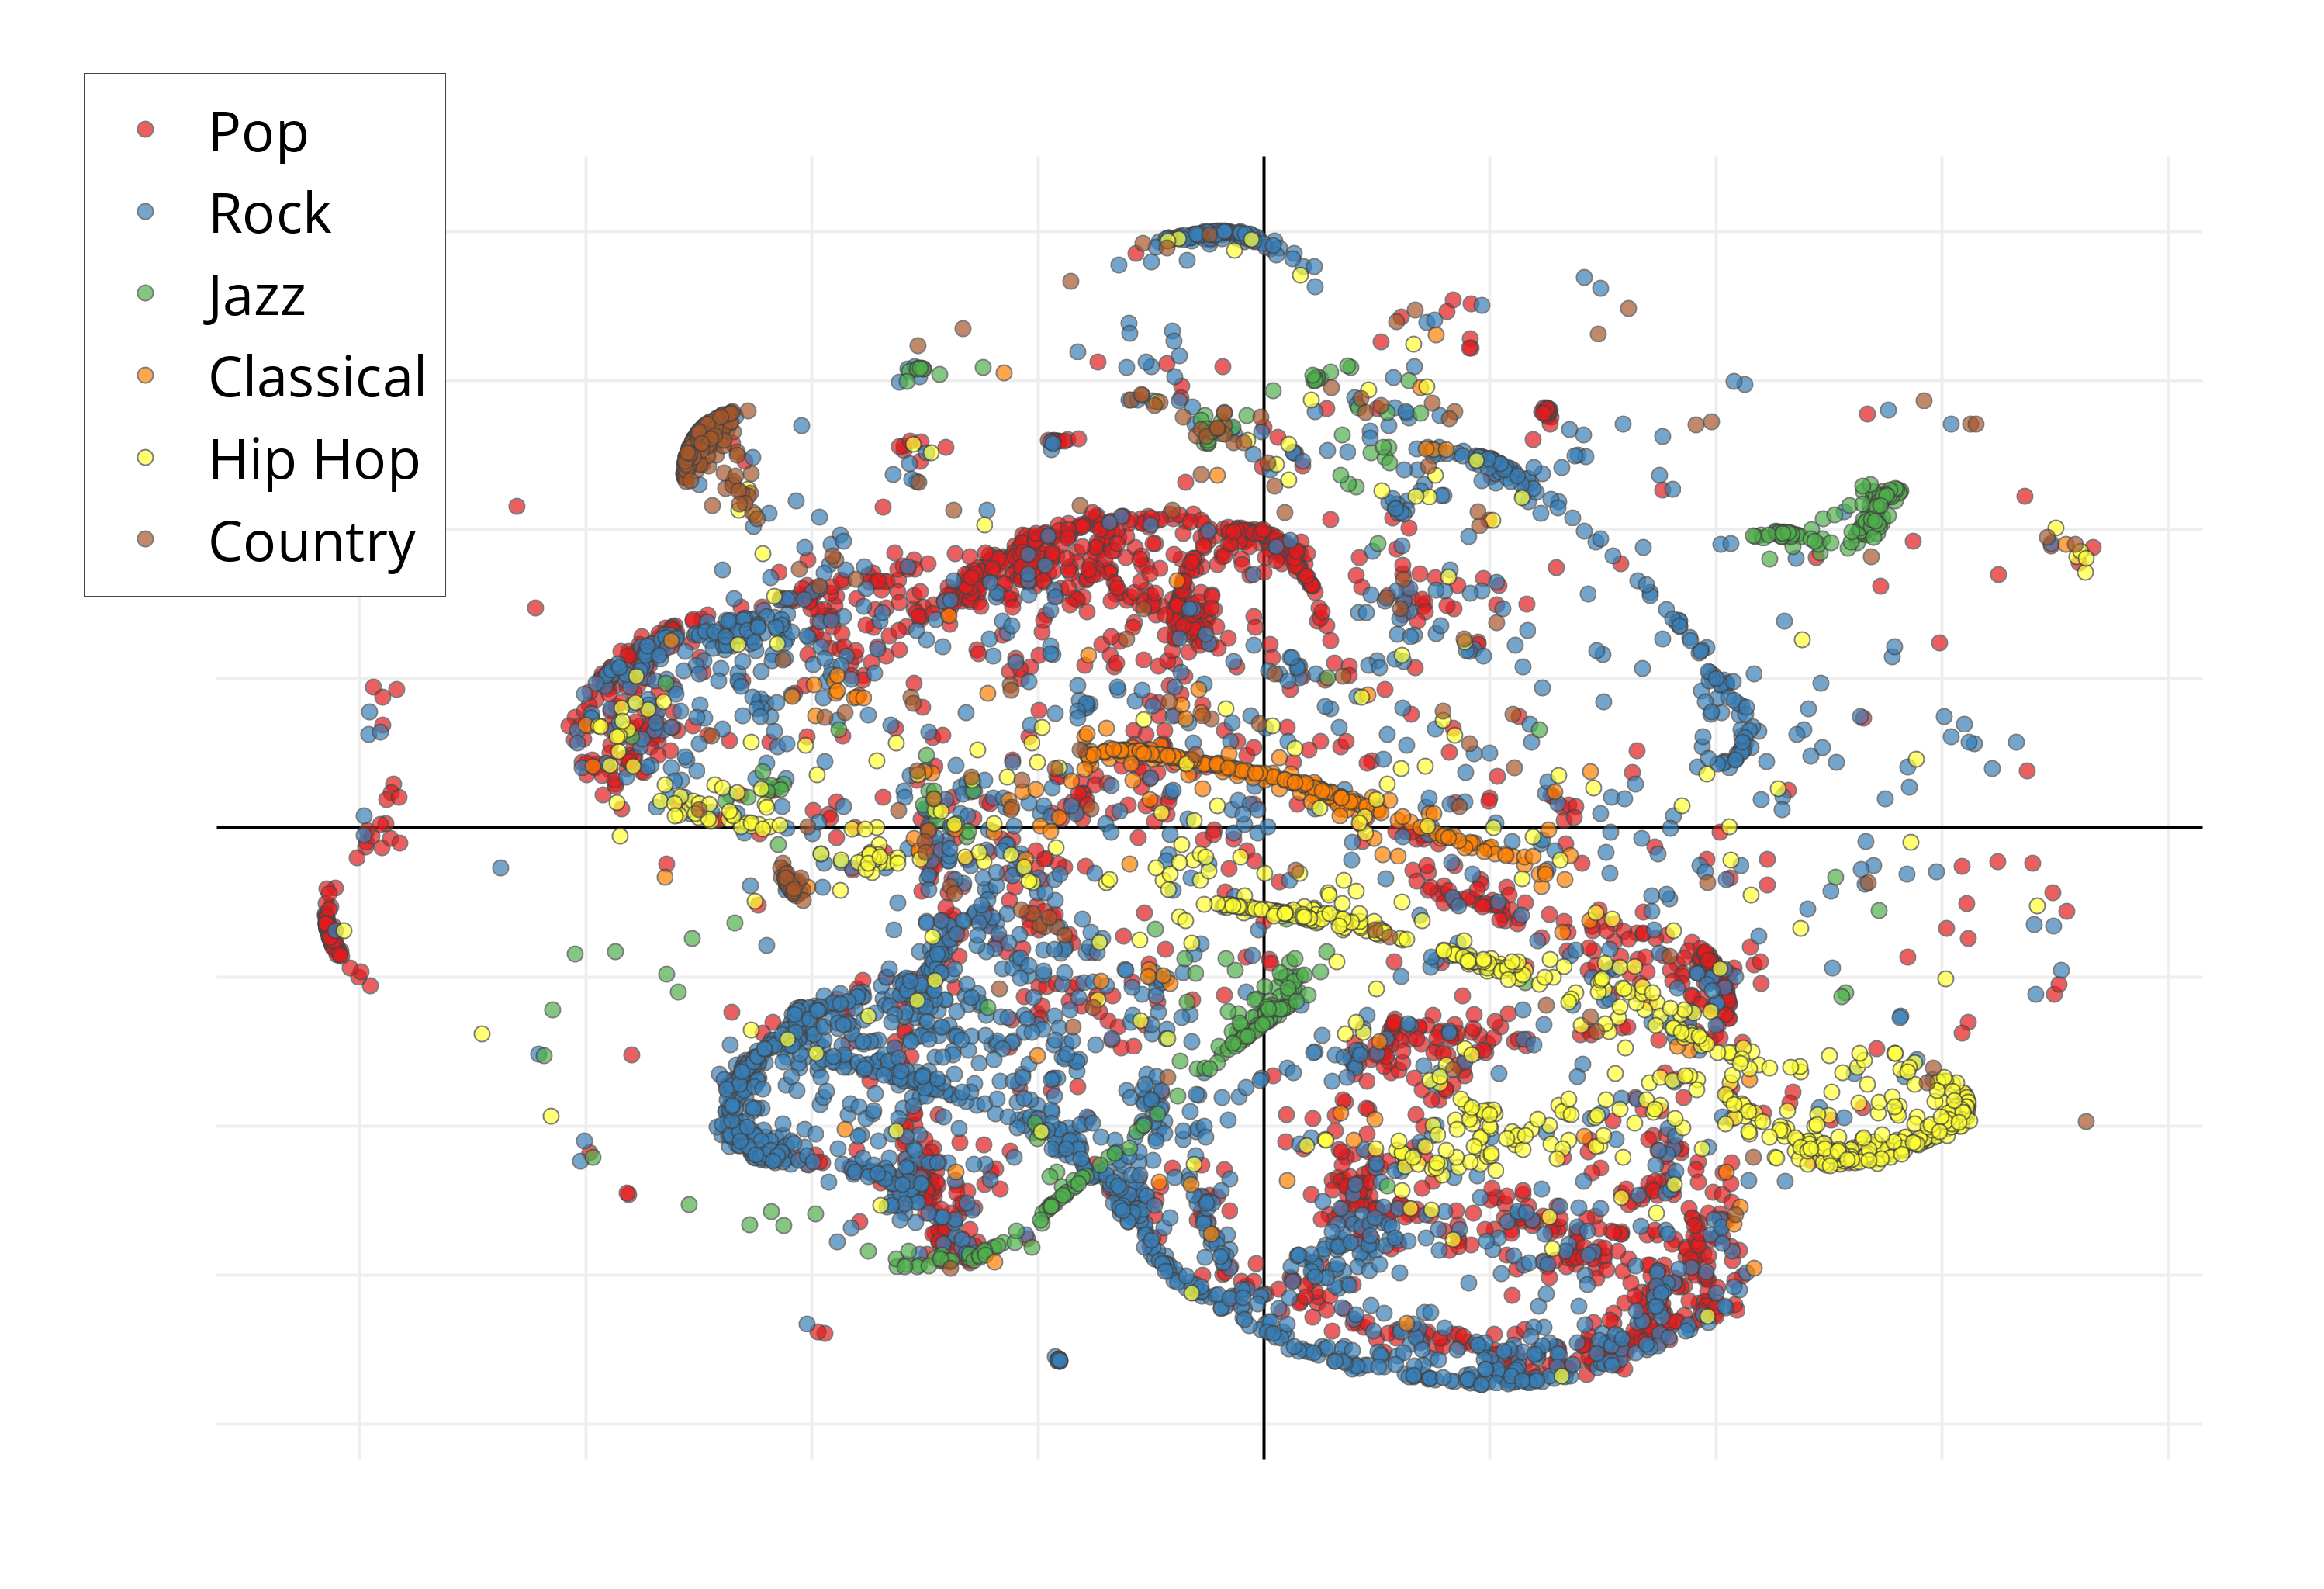
\includegraphics{figs/tSNEfig.png}
	}		
	\vspace{-0.8cm}
	\caption{tSNE embedding of artist parameters. The figure shows a complex manifold that could not be captured by modeling higher levels of the taxonomy alone.}
	\label{tSNEfig}
%	\vspace{-0.3cm}
\end{figure}
 \GL{Doesnt the setup of the model ensure this behavior? Not sure this justifies any assumptions, more like reflects the assumptions of our model IMO. } 

%We present this figure as further evidence that the learned parameters capture inherent semantics in the domain \GL{this final sentence is problematic, how do we see this from the figure?} \noam{Agree.}.

\subsection{Anecdotal Results}

\begin{table}

\centering
\scalebox{0.5}{
\begin {tabular}{lll}%
\\%
\textbf {Track Title} & \textbf {Artist Name} & \textbf {Album Name}\\
 \midrule \multicolumn {3}{c}{\textbf {Artist Seed: Rihanna (Pop Singer)}} \\ 
 \midrule Yeah, I Said It&Rihanna&ANTI\\%
Birthday&Katy Perry&PRISM\\%
She Will Be Loved&Maroon 5&Songs About Jane\\%
I'm Real&Jennifer Lopez&J. Lo\\%
Yeah! (feat. Lil' Jon \& Ludacris)&Usher&Confessions\\%
\midrule \multicolumn {3}{c}{\textbf {Artist Seed: Wes Montogomery (Jazz Guitarist)}} \\ \midrule Bumpin' On Sunset&Wes Montgomery&Wes Montgomery: Finest Hour\\%
The Natives Are Restless Tonight&Horace Silver&Song For My Father\\%
I Remember Clifford&Lee Morgan&The Ultimate Collection\\%
Gee Baby, Ain't I Good To You&Kenny Burrell&Midnight Blue\\%
West Coast Blues&Wes Montgomery&The Jazz Effect - Wes Montgomery\\%
\midrule \multicolumn {3}{c}{\textbf {Artist Seed: Itzhak Perlman (Classical Violinist)}} \\ \midrule Il Postino: Theme (Instrumental)&Itzhak Perlman&Cinema Serenade\\%
Brahms: Hungarian Dance No.5&Nicola Benedetti&The Violin\\%
Violin Concerto No. 2 in E Major ..&Joshua Bell&Bach\\%
Piezas Caracteristicas, Op. 92&John Williams&The Ultimate Guitar Collection\\%
Adagio for Strings&Leonard Bernstein&Barber's Adagio ...\\\bottomrule %
\end {tabular}%
}
\caption{ Anecdotal results: shows the top 5 tracks in the playlist generated for several seed seed artists.} 
\label{anecdotalResultsTable}
\end{table}

To give a flavor of the type of output generated by the proposed approach Table \ref{anecdotalResultsTable} shows the top five tracks in the playlist for three very different seed artists. Notably, using the \textit{Pop} star \textit{Rihanna} as a seed results in a playlist composed of tracks by other \textit{Pop} artists which do not necessarily sound similar to \textit{Rihanna}. For the \textit{Jazz} and \textit{Classical} seed artists, we see that the playlist is not only composed of tracks from the same genre of the artist, but further many tracks include instrumentation similar to that of the seed artist. These playlists are generated by a variant of the algorithm proposed in this work which currently powers the Microsoft's \textit{Groove Music} service.



\GLw{Removed section on AB Testing...}
%\subsection{Online A/B Testing}
%We performed an A/B experiment comparing a variant of the model described above with Groove's previous playlist algorithm. The experiment was conducted by randomly assigning users to buckets and measuring online metrics designed to quantify user satisfaction and engagement. Specifically, we consider \textit{Average Session Length} (ASL), and \textit{User Average Skip Ratio} (UASR). ASL is the listening time elapsed in a single radio session, averaged over all such sessions. UASR is a the ratio of skipped tracks to tracks that were played to completion averaged over all users. The approach in this paper was able to outperform the baseline on both metrics showing an increase of $4.21\%$ in ASL and a $5.76\%$ decrease in UASR.  


%\begin{table}[h]
%\centering
%\begin{tabular}{|c|c|c|}
% \hline
%  KPI & Improvement & P-value \\
% \hline
% ASL & $4.21\%$ & $0$ \\
% \hline
% UASR & $5.76\%$ & $0$\\
% \hline
%\end{tabular}
%    \caption{This table shows the improvement and p-value per measured KPI.}
%    \label{tabel:kpis}
%\end{table}

%\subsection{Anecdotal Comparison}
%
%\begin{table}[H]
%\centering
%\begin{tabular}{ | l | l |l| }
%
%  \hline			
%  Our Algorithm & EchoNest & Last.FM \\
%  \hline
%  Madonna & Shlomo Artzi & John Coltrane\\
%  Cher &  &  \\
%    \hline
%\end{tabular}
%    \caption{Seed Artist:Kylie Minouge}
%\end{table} 





%\vspace{-2mm}    
 \section{Practical Considerations}
 In this section we offer some discussion on ideas that allow the application of the model proposed in this paper to a real-world system serving a large number of users.

The playlist is constructed sequentially by picking the next track using the ranking induced by $\hat{r}_m$ from (\ref{eq:PredictionApproximation}). However, in practice we first apply two important heuristics. First, since it is impractical to consider the tens of millions of tracks in the Groove music catalog, we first pre-compute a candidate list of $M \approx 1,000$ tracks for each possible seed artist.
The candidate list for an artist $a^*$ consists of $a^*$'s tracks and tracks from artists similar to $a^*$. Second, we define a Boltzmann distribution over the $m=1 \dots M$ tracks with each candidate track having a probability given by $p_m=\frac{e^{s \cdot \hat{r}_m}}{\sum_{i=1}^M e^{s \cdot \hat{r}_i}}$, where $s$ is a tunable parameter. The next track is chosen randomly with probability $p_m$. This scheme ensures a degree of diversity, controlled by $s$, between multiple instances of similar playlists. This type of randomization also acts as an exploration mechanism, allowing labels to be collected from areas where the model is less certain. This reduces the feedback loop effect when learning future models based on user interactions with the system.



An advantage of the Bayesian setup described in this work is that it is fairly straightforward to adjust the model parameters in an online fashion. For example, consider the scenario where a playlist user skips several tracks in a row. Our approach could be extended to update the user parameter vector given these additional explicit negatives, before computing the next track selection.

\noam{I think the discussion about hyper-params better fit in the model section. However, I prefer to drop it for now because I don't think it strengthen the paper.}
%When setting hyper-parameters, we fixed them to $\alpha=\beta=1$ as we observed that results are robust to this setting. For completeness, hyper-parameters can also be tuned with cross-validation. \GL{This should be stated in the model section if it pertains to the experiments. Though, i dont think it has too much added value or insight to justify being included at all}
Finally, our model is designed for implicit feedback signals, as these are more common in commercial settings, hence the use of binary labels. However, in some scenarios explicit user ratings are known. Support for such scenarios can be achieved by modifying the likelihood term of our model (in (\ref{eq:likelihood})) and re-deriving the update equations.
\GL{is anything missing here? some discussion of the settings of the hyper parameters and the "active" range of the logistic function as per ulrich's suggestion perhaps?} \noam{This can go on forever... :)  I think these good points suffice.} \SBE{I think the hyperparameter discussion is important, and tried to keep it short.}
%\section{Discussion}
%    \begin{itemize}
  \item Intuition Behind Results
  \item Qualitative comparison of single song vs whole playlist optimization
  \item ??
\end{itemize}

%\vspace{-2mm}
\section{Conclusion}
    This work describes a model for playlist generation designed for Microsoft's Groove music service. The model incorporates per-artist parameters in order to capture the unique characteristics of an artist's playlists. The domain taxonomy of genres, sub-genres and artists is utilized in order to allow training examples from one artist to inform predictions of other related artists. Hence, the model offers good predictions even when a playlist is requested for a ``seed'' artist for whom little (or even no) historical information is available. Furthermore, the proposed model is endowed with the capacity to capture particular user preferences for those users who are frequent playlist requesters, enabling a personalized playlist experience. %For ``cold'' users who are using the system for the first few times, the semantics of the ``seed'' artist enable the model to provide a good playlist without relying only on user information.

A variational inference learning algorithm is applied and a detailed description of the update steps of each parameter is provided in Section~\ref{sec:OurModel}. %This algorithm is run iteratively, until the convergence of a bound on the variational free energy.
The evaluations in Section~\ref{sec:experiments} show the benefit of using the domain taxonomy as well as the personalization components for the playlist generation task at hand. Finally, an online experiment is described showing a significant increase in user listening time and a significant reduction in skipped tracks. %Some practical considerations for implementing the proposed approach at scale on a real-world system are discussed in the final section.


\label{sec:conclusion}

%\vspace{-2mm}
\bibliographystyle{abbrv}
\bibliography{Radio_Bib}


\end{document}
